\documentclass[a4paper,11pt,oneside]{report}

\usepackage[T1]{fontenc}
\usepackage[utf8]{inputenc}
\usepackage[english]{babel}
\usepackage[a4paper,margin=25mm]{geometry}
\usepackage{lmodern}
\usepackage{microtype}
\usepackage{graphicx}
\usepackage{booktabs}
\usepackage{longtable}
\usepackage{array}
\usepackage{enumitem}
\usepackage{siunitx}
\usepackage{xcolor}
\usepackage{amsmath}
\usepackage{hyperref}
\usepackage{cleveref}
\usepackage{fancyhdr}
\usepackage{caption}
\usepackage{float}

\graphicspath{{figures/SystemViews/}{figures/ReferenceViews/}{figures/SoftwareViews/}{figures/HardwareViews/}{figures/ValidationViews/}}

\hypersetup{
  colorlinks=true,
  linkcolor=blue,
  citecolor=blue,
  urlcolor=blue,
  pdftitle={ND280 Magnetic Field Monitoring System - Technical Design Report},
  pdfauthor={Stefano Levorato}
}

\pagestyle{fancy}
\setlength{\headheight}{14pt}
\fancyhf{}
\lhead{ND280 Magnetic Field Monitoring System}
\rhead{TDR v0.6}
\cfoot{\thepage}

\setcounter{tocdepth}{2}
\setcounter{secnumdepth}{3}

\title{
  \vspace{1.5cm}
  \textbf{ND280 Magnetic Field Monitoring System}\\[0.5cm]
  \Large Technical Design Report\\[0.5cm]
  \large Version 0.6
}
\author{
  Stefano Levorato\\
  INFN -- Laboratori Nazionali di Legnaro
}
\date{August 2026}

\begin{document}
\maketitle
\vfill
\begin{center}
\textbf{Internal development document}
\end{center}
\newpage

\chapter*{Document Control}
\addcontentsline{toc}{chapter}{Document Control}
\begin{tabular}{ll}
\toprule
Document & ND280 Magnetic Field Monitoring System -- Technical Design Report \\
Version & 0.6 \\
Status & Draft for internal review \\
Author & Stefano Levorato \\
Institution & INFN -- Laboratori Nazionali di Legnaro \\
Repository & \url{https://github.com/stefanolevorato/ND280-Magnetic-Field-Monitoring-System} \\
\bottomrule
\end{tabular}

\vspace{1cm}
\section*{Revision History}
\begin{tabular}{llll}
\toprule
Version & Date & Author & Description \\
\midrule
0.1 & August 2026 & S. Levorato & Initial LaTeX project structure \\
0.2 & August 2026 & S. Levorato & Scientific motivation and bibliography \\
0.3 & August 2026 & S. Levorato & System Views and Chapters 4--5 completed \\
0.4 & August 2026 & S. Levorato & Added monitor long-duration evidence and Rev.A hardware render \\
0.5 & August 2026 & S. Levorato & Added calibration and metrological characterization strategy \\
0.6 & August 2026 & S. Levorato & Added preliminary stability characterization and ROOT analysis plots \\
\bottomrule
\end{tabular}

\clearpage
\tableofcontents
\clearpage
\listoffigures
\clearpage
\listoftables
\clearpage

\chapter{Introduction}

\section{Background and Motivation}

The ND280 Magnetic Field Monitoring System is an instrumentation project developed by the Istituto Nazionale di Fisica Nucleare (INFN) with the objective of designing, implementing and validating a distributed magnetic-field monitoring infrastructure for the ND280 detector at the Japan Proton Accelerator Research Complex (J-PARC).

The project originates from the need for a compact, modular and scalable monitoring system capable of continuously monitoring the magnetic field at multiple locations inside the detector while providing long-term stability, comprehensive diagnostic capabilities and straightforward integration with the experiment control infrastructure.

Commercial magnetic-field monitoring systems generally do not satisfy the geometrical, mechanical and integration constraints required for the ND280 Near Detector of the T2K experiment, installed inside the C-shaped UA1 magnet. For this reason, a dedicated monitoring system has been specifically designed and developed.

The proposed system is based on intelligent acquisition nodes, each capable of locally acquiring, processing, validating and transmitting magnetic-field measurements while operating autonomously. Each node performs local sensor management, data acquisition, calibration, diagnostics and health monitoring before making the acquired information available to higher-level controllers.

\section{Design Philosophy}

The overall architecture has been intentionally developed following a modular engineering approach in which hardware, embedded firmware, desktop software and technical documentation evolve together under version control.

The system has been designed by separating hardware abstraction, device drivers, acquisition services and application logic. This modular organization minimizes software dependencies and allows future hardware revisions to reuse the same firmware architecture with minimal modifications.

The desktop application, referred to throughout this document as the \textit{ND280 Monitor}, has been developed as an engineering tool supporting commissioning, diagnostics, calibration, visualization and long-term data logging.

The development follows an incremental engineering methodology in which every hardware revision is accompanied by the corresponding firmware, desktop software and validation campaign before introducing additional functionality.

This approach minimizes technical risk, simplifies debugging activities and preserves software compatibility throughout the evolution of the project.

\section{Project Evolution}

The development started from a Reference Single-Sensor Node whose purpose was the validation of the complete acquisition chain, including hardware, firmware, communication protocol and monitoring software.

Once the architecture had been validated through extensive functional and long-duration tests, the project evolved towards the design of an Eight-Sensor Multiplexing Node based on the Texas Instruments TCA9548A I\textsuperscript{2}C multiplexer.

The new hardware architecture extends the acquisition capability from one to eight magnetic sensors while preserving the existing NodeOS architectural principles.

The long-term objective of the project is the realization of a distributed magnetic-field monitoring infrastructure composed of multiple intelligent acquisition nodes interconnected through a segmented communication network and coordinated by a dedicated controller.

\section{Scope of this Document}

This Technical Design Report describes the complete design of the ND280 Magnetic Field Monitoring System, from the validated Reference Single-Sensor Node to the current Eight-Sensor Multiplexing Node and the future distributed acquisition architecture.

The document presents the hardware design, embedded firmware architecture (NodeOS), communication protocol, desktop monitoring software, validation campaign, engineering decisions and future development roadmap.

The purpose of this document is not only to describe the current implementation but also to record the engineering rationale behind the adopted architectural choices, providing a technical reference for future hardware revisions and software developments.

\chapter{Scientific Motivation}

\section{Experimental Context}

The T2K experiment is a long-baseline neutrino-oscillation experiment located at J-PARC, Japan. Its off-axis near detector, ND280, is installed approximately \SI{280}{m} from the neutrino production target and operates inside a magnet providing a nominal field of approximately \SI{0.2}{T}. The neutrino beam is first measured by the near detectors, including ND280, and then travels to the far detector, Super-Kamiokande.

The two new High-Angle Time Projection Chambers (HA-TPCs) were installed as part of the ND280 upgrade, which was completed at J-PARC in 2024 \cite{HATPCPerformance}.

ND280 is installed inside the UA1/NOMAD magnet, which provides a nominal magnetic field of approximately \SI{0.2}{T}. The magnetic field allows ND280 to bend charged-particle trajectories, determine the sign of the particle charge, and measure the momentum of particles produced in neutrino interactions \cite{TPCWorkshop,NewTPCsGDR,ND280Review}.

\section{Magnetic Field}

A TPC does not measure the momentum of a charged particle directly. It measures a sequence of points along the particle trajectory. In a magnetic field, the trajectory is curved, and the curvature is used to infer the momentum and the sign of the charge.

For a charged particle in a uniform magnetic field, the transverse momentum is approximately related to the radius of curvature by
\begin{equation}
 p_T\,[\si{GeV/c}] \simeq 0.3\,|q|\,B\,[\si{T}]\,R\,[\si{m}],
 \label{eq:pt}
\end{equation}
where $p_T$ is the transverse momentum, $q$ is the charge in units of the elementary charge, $B$ is the magnetic-field strength, and $R$ is the radius of curvature.

In the real reconstruction, the track fit should use the three-dimensional field map
\begin{equation}
 \vec{B}(x,y,z),
 \label{eq:bmap}
\end{equation}
rather than only the nominal central value. A dedicated device was developed to measure and map the magnetic field of the ND280 magnet \cite{MagneticFieldDevice}.

\section{Magnetic Field at ND280}

The value of \SI{0.2}{T} is a nominal or average value. The actual magnetic field can vary spatially and can include components transverse to the nominal field direction. Variations may occur near magnet openings, detector structures, and the boundaries of the active TPC volume.

For track reconstruction, the relevant quantity is related to the field integrated along the trajectory. Schematically,
\begin{equation}
 \Delta\phi \propto \int B_{\perp}\,\mathrm{d}l,
 \label{eq:integral}
\end{equation}
where $B_{\perp}$ is the component responsible for the measured bending and the integral is taken along the track.

A recent HA-TPC performance paper mentions a magnetic-field map obtained from measurements performed in 2009 in the region of the vertical TPCs \cite{HATPCPerformance}. This makes it important to verify that the map used for the HA-TPC reconstruction is representative of the actual position and configuration of the upgraded chambers.

\section{Impact on Momentum Reconstruction}

If the field is treated as uniform and the relative uncertainty on its scale is $\delta B/B$, then, for a fixed measured curvature,
\begin{equation}
 \frac{\delta p_T}{p_T} \simeq \frac{\delta B}{B}.
 \label{eq:scale}
\end{equation}

Thus, a one-percent systematic error in the magnetic-field scale produces approximately a one-percent systematic error in the momentum scale. This is a momentum-scale uncertainty and is distinct from the statistical momentum resolution, which is also affected by the number and precision of measured points, diffusion, and multiple scattering.

An inaccurate field map can produce several effects:
\begin{itemize}[leftmargin=*]
  \item a bias in the reconstructed momentum scale;
  \item a position-dependent or angle-dependent momentum bias;
  \item a degradation of the momentum resolution;
  \item differences between the reconstructed response of positive and negative tracks;
  \item a lower reliability of the charge-sign determination.
\end{itemize}

These effects can propagate to the reconstructed lepton momentum and angle, neutrino-energy estimators, event classification, and the systematic uncertainties used in the T2K oscillation analysis. ND280 is used to constrain uncertainties in the neutrino flux and neutrino-interaction models before oscillation \cite{HATPCPerformance}.

\section{Specific Relevance for the HA-TPCs}

The HA-TPCs were designed to reconstruct particles emitted at large angles relative to the neutrino-beam direction. They are positioned above and below the Super-FGD. The coordinate system used for ND280 is defined with the $x$ axis parallel to the main component of the magnetic field, the $y$ axis opposite to the direction of gravity, and the $z$ axis along the incoming neutrino beam \cite{HATPCPerformance}.

The magnetic-field map is particularly important for the HA-TPCs for the following reasons:
\begin{enumerate}[leftmargin=*]
  \item Tracks can cross different regions of the HA-TPC, so the reconstruction depends on the field along the full track.
  \item Components of the field that are not aligned with the nominal direction can modify the three-dimensional curvature.
  \item Some high-angle particles may have a shorter track lever arm, making the momentum more sensitive to field-scale and alignment errors.
  \item The magnetic field can affect electron transport and transverse charge diffusion in the TPC. These effects must be separated from distortions caused by the electric field, field-cage geometry, gas properties, and Micromegas response.
  \item The field map enters both the detector simulation and the track-reconstruction algorithms.
\end{enumerate}

\section{Recommended Checks for an HA-TPC Field Study}

A dedicated study should verify:
\begin{enumerate}[leftmargin=*]
  \item the three-dimensional field map used by the reconstruction software;
  \item whether the map is based on direct measurements, magnetostatic simulations, or both;
  \item coverage of the complete HA-TPC active volume;
  \item the absolute accuracy of the field scale;
  \item the accuracy of the $B_x$, $B_y$, and $B_z$ components;
  \item the alignment between the field-map coordinate system, the magnet, and the HA-TPCs;
  \item agreement between cosmic-ray data and simulation;
  \item comparisons of positive and negative tracks;
  \item reconstructed momentum as a function of position, angle, and charge;
  \item propagation of the field uncertainty into the final physics analysis.
\end{enumerate}

\section{Implication for the Monitoring System}

Measuring the magnetic field in ND280 is necessary because the momentum and charge sign are obtained from the curvature of charged-particle tracks in the TPC. For the HA-TPCs, the nominal value of \SI{0.2}{T} is not sufficient. A three-dimensional magnetic-field map is required in the actual volume occupied by the chambers.

The leading direct effect of a field-scale error is a bias in the reconstructed momentum. To first order,
\begin{equation}
 \frac{\delta p}{p} \simeq \frac{\delta B}{B}.
\end{equation}

An incorrectly modelled field non-uniformity or field direction can additionally degrade the momentum resolution, introduce artificial dependencies on position and angle, and reduce the reliability of charge determination.

These considerations provide the scientific motivation for the development of a dedicated distributed magnetic-field monitoring system capable of collecting stable, spatially distributed and traceable magnetic-field measurements over long operating periods.

\chapter{System Requirements and Design Drivers}

 
\section{Overview}

The ND280 Magnetic Field Monitoring System has been designed to satisfy a combination of scientific, functional, operational and engineering requirements.

The requirements defined in this chapter provide the reference framework for the hardware architecture, NodeOS firmware, ND280 Monitor application, validation activities and future system extensions.

Each requirement is assigned a unique identifier to support traceability throughout the development and qualification process.

\section{Functional Requirements}

\begin{longtable}{p{18mm}p{106mm}p{23mm}}
	\toprule
	ID & Requirement & Status \\
	\midrule
	
	REQ-001 &
	The system shall continuously acquire the three magnetic-field components $B_x$, $B_y$ and $B_z$. &
	Verified \\
	
	REQ-002 &
	The system shall acquire the temperature measured by each magnetic sensor. &
	Verified \\
	
	REQ-003 &
	Each acquisition node shall provide a unique hardware identifier. &
	Verified \\
	
	REQ-004 &
	Calibration parameters shall be stored in non-volatile memory and shall survive power cycling. &
	Verified \\
	
	REQ-005 &
	Each acquisition node shall automatically recover from a firmware stall through hardware watchdog supervision. &
	Verified \\
	
	REQ-006 &
	Each acquisition node shall provide diagnostic information including acquisition statistics, communication errors and reset cause. &
	Verified \\
	
	REQ-007 &
	The monitoring software shall provide real-time visualization of magnetic-field and temperature measurements. &
	Verified \\
	
	REQ-008 &
	The monitoring software shall provide persistent data logging for long-duration acquisitions. &
	Verified \\
	
	REQ-009 &
	The command interface shall reject malformed or unrelated serial traffic without disrupting the acquisition process. &
	Verified \\
	
	REQ-010 &
	The magnetic-field measurement range shall provide adequate headroom with respect to the nominal ND280 magnetic field of approximately \SI{0.2}{T}. &
	Verified \\
	
	REQ-011 &
	The local acquisition architecture shall support up to eight TMAG5273A2 sensors connected to a single intelligent node. &
	Rev.A design \\
	
	REQ-012 &
	The system architecture shall support multiple acquisition nodes connected through a common inter-board communication network. &
	In development \\
	
	REQ-013 &
	The distributed architecture shall support up to 32 acquisition boards, corresponding to a maximum of 256 magnetic sensors. &
	Design target \\
	
	REQ-014 &
	The same acquisition-board hardware shall be capable of operating either as a NODE or as a COORDINATOR. &
	Rev.A design \\
	
	REQ-015 &
	The NODE or COORDINATOR operating role shall be selected through a dedicated hardware configuration input. &
	Rev.A design \\
	
	\bottomrule
\end{longtable}

\section{Reliability Requirements}

\begin{longtable}{p{18mm}p{106mm}p{23mm}}
	\toprule
	ID & Requirement & Status \\
	\midrule
	
	REL-001 &
	The acquisition process shall continue without operator intervention during normal long-duration operation. &
	Verified \\
	
	REL-002 &
	A communication error shall not corrupt the internal measurement state of the acquisition node. &
	Verified \\
	
	REL-003 &
	Invalid EEPROM contents shall be detected and replaced by safe default calibration values. &
	Verified \\
	
	REL-004 &
	The firmware shall record the cause of the most recent microcontroller reset. &
	Verified \\
	
	REL-005 &
	The external I\textsuperscript{2}C interface of each board shall remain disabled during microcontroller reset and early boot. &
	Rev.A design \\
	
	REL-006 &
	The inter-board communication architecture shall electrically segment successive sections of the I\textsuperscript{2}C network. &
	Rev.A design \\
	
	\bottomrule
\end{longtable}

\section{Engineering Design Drivers}

The system architecture has also been influenced by a number of engineering design drivers that are not purely functional requirements but are considered essential for maintainability and future system evolution.

\begin{itemize}[leftmargin=*]
	
	\item \textbf{Modularity.}
	Hardware abstraction, device drivers, acquisition services and application logic shall remain separated.
	
	\item \textbf{Firmware reuse.}
	A new hardware revision should not require a complete redesign of NodeOS.
	
	\item \textbf{Deterministic embedded behaviour.}
	Dynamic memory allocation is avoided in the embedded firmware.
	
	\item \textbf{Hardware-defined identity.}
	The Node ID is determined by hardware configuration rather than by software or EEPROM contents.
	
	\item \textbf{Hardware-defined operating role.}
	The NODE/COORDINATOR role is determined by a dedicated hardware jumper.
	
	\item \textbf{Local data processing.}
	Each intelligent node performs sensor acquisition, averaging, calibration and diagnostics locally before data are transferred to higher-level controllers.
	
	\item \textbf{Independent subsystem validation.}
	Each hardware and software subsystem should be testable independently.
	
	\item \textbf{Incremental qualification.}
	New functionality is introduced only after the previous development stage has been validated.
	
	\item \textbf{Single-board architecture.}
	Whenever practical, NODE and COORDINATOR operation should use the same PCB and bill of materials.
	
\end{itemize}


\section{Calibration and Metrological Requirements}

The ND280 Magnetic Field Monitoring System is not intended to replace a dedicated high-precision magnetic-field mapping instrument. Its primary purpose is distributed, long-term monitoring of the magnetic field and the detection of spatial or temporal variations relevant to detector operation. Nevertheless, the usefulness of such a monitor depends on the measurements being sufficiently stable, reproducible and comparable between sensors and acquisition nodes.

A recent calibration study of a dedicated three-dimensional Hall sensor card developed at CERN illustrates the principal error sources that can affect Hall-based vector measurements, including offset, temperature dependence, non-linearity, cross-axis effects and mechanical or angular misalignment. The same study emphasizes that a dedicated calibration procedure is required when high measurement accuracy is needed \cite{MessnerHallCalibration}. The absolute performance target of that system is substantially more demanding than required for the ND280 monitoring application; however, the underlying metrological methodology is directly relevant to the present project.

The following requirements are therefore adopted for the calibration and characterization programme of the ND280 monitoring nodes:

\begin{longtable}{p{18mm}p{106mm}p{23mm}}
\toprule
ID & Requirement & Status \\
\midrule

CAL-001 &
Each magnetic sensor shall have an individually identifiable calibration data set. &
Design target \\

CAL-002 &
The calibration model shall support correction of per-axis offset and sensitivity and shall be extensible to cross-axis and alignment corrections if required by characterization data. &
Design target \\

CAL-003 &
Calibration coefficients shall be stored in non-volatile memory together with a calibration format or version identifier. &
Partially implemented \\

CAL-004 &
The calibration procedure shall characterize the temperature dependence of the magnetic-field measurement over the expected operating temperature range. &
Planned \\

CAL-005 &
The calibration campaign shall evaluate sensor-to-sensor and board-to-board reproducibility using multiple independently assembled units. &
Planned \\

CAL-006 &
The calibration model shall be validated over the magnetic-field range relevant to ND280 operation and shall provide adequate margin around the nominal field of approximately \SI{0.2}{T}. &
Planned \\

CAL-007 &
The system shall preserve the raw or minimally processed sensor information required to repeat calibration studies and to evaluate alternative correction models offline. &
Design target \\

CAL-008 &
The calibration procedure and its resulting coefficients shall be traceable through documented calibration conditions, sensor identity, calibration date and validation results. &
Planned \\

\bottomrule
\end{longtable}

The calibration model will intentionally be kept no more complex than justified by the characterization results. The current offset-and-gain representation therefore remains a valid first-level model. A full three-dimensional correction matrix and explicit temperature terms will be introduced only if measurements demonstrate that they provide a significant improvement in the operating range of the monitoring system.

\section{Scalability}

The system has been intentionally developed through successive levels of complexity:

\begin{enumerate}[leftmargin=*]
	
	\item Reference Single-Sensor Node;
	
	\item Eight-Sensor Multiplexing Node;
	
	\item Distributed Multi-Board Acquisition System;
	
	\item Complete detector monitoring infrastructure.
	
\end{enumerate}

Each validated development stage provides the reference platform for the following stage.

The Reference Single-Sensor Node validates the complete acquisition chain and the NodeOS architecture.

The Eight-Sensor Multiplexing Node extends local acquisition capability by introducing the TCA9548A while preserving the existing firmware architecture.

The distributed system introduces inter-board communication and coordinator functionality without modifying the local sensor-acquisition concept.

\section{Verification Strategy}

Each requirement shall be associated with one or more verification activities.

Verification methods include:

\begin{itemize}[leftmargin=*]
	
	\item schematic and PCB design review;
	
	\item firmware unit and integration tests;
	
	\item communication protocol tests;
	
	\item watchdog and reset-recovery tests;
	
	\item EEPROM persistence tests;
	
	\item sensor acquisition tests;
	
	\item long-duration stability tests;
	
	\item inter-board communication tests;
	
	\item final detector-level characterization.
	
\end{itemize}

A Requirements Traceability Matrix will be maintained as part of the validation documentation and will associate each requirement with the corresponding implementation and verification evidence.

\section{Summary}

The requirements defined in this chapter establish the functional and engineering framework of the ND280 Magnetic Field Monitoring System.

The design prioritizes measurement continuity, robustness, modularity, scalability and long-term maintainability. These requirements directly motivate the system architecture described in the following chapter.
\chapter{System Architecture Views}
\label{chap:system-architecture}

\section{Purpose of the Architecture Views}

The architecture of the ND280 Magnetic Field Monitoring System is described through a set of complementary \emph{System Views}. Each view answers one specific engineering question and intentionally omits implementation details that are not required at that level of abstraction.

This representation separates the overall system structure, the acquisition-node concept, the embedded-software organization, the measurement-processing path and the engineering evolution of the project. The same views can therefore remain valid across future hardware revisions even when individual devices or implementation details change.

\section{Overall System Architecture}

The complete monitoring infrastructure is organized as a hierarchy of intelligent acquisition nodes coordinated by a higher-level controller. The desktop application provides configuration, diagnostics, visualization and persistent data logging, while magnetic-field acquisition and preprocessing remain local to each node.

\begin{figure}[htbp]
  \centering
  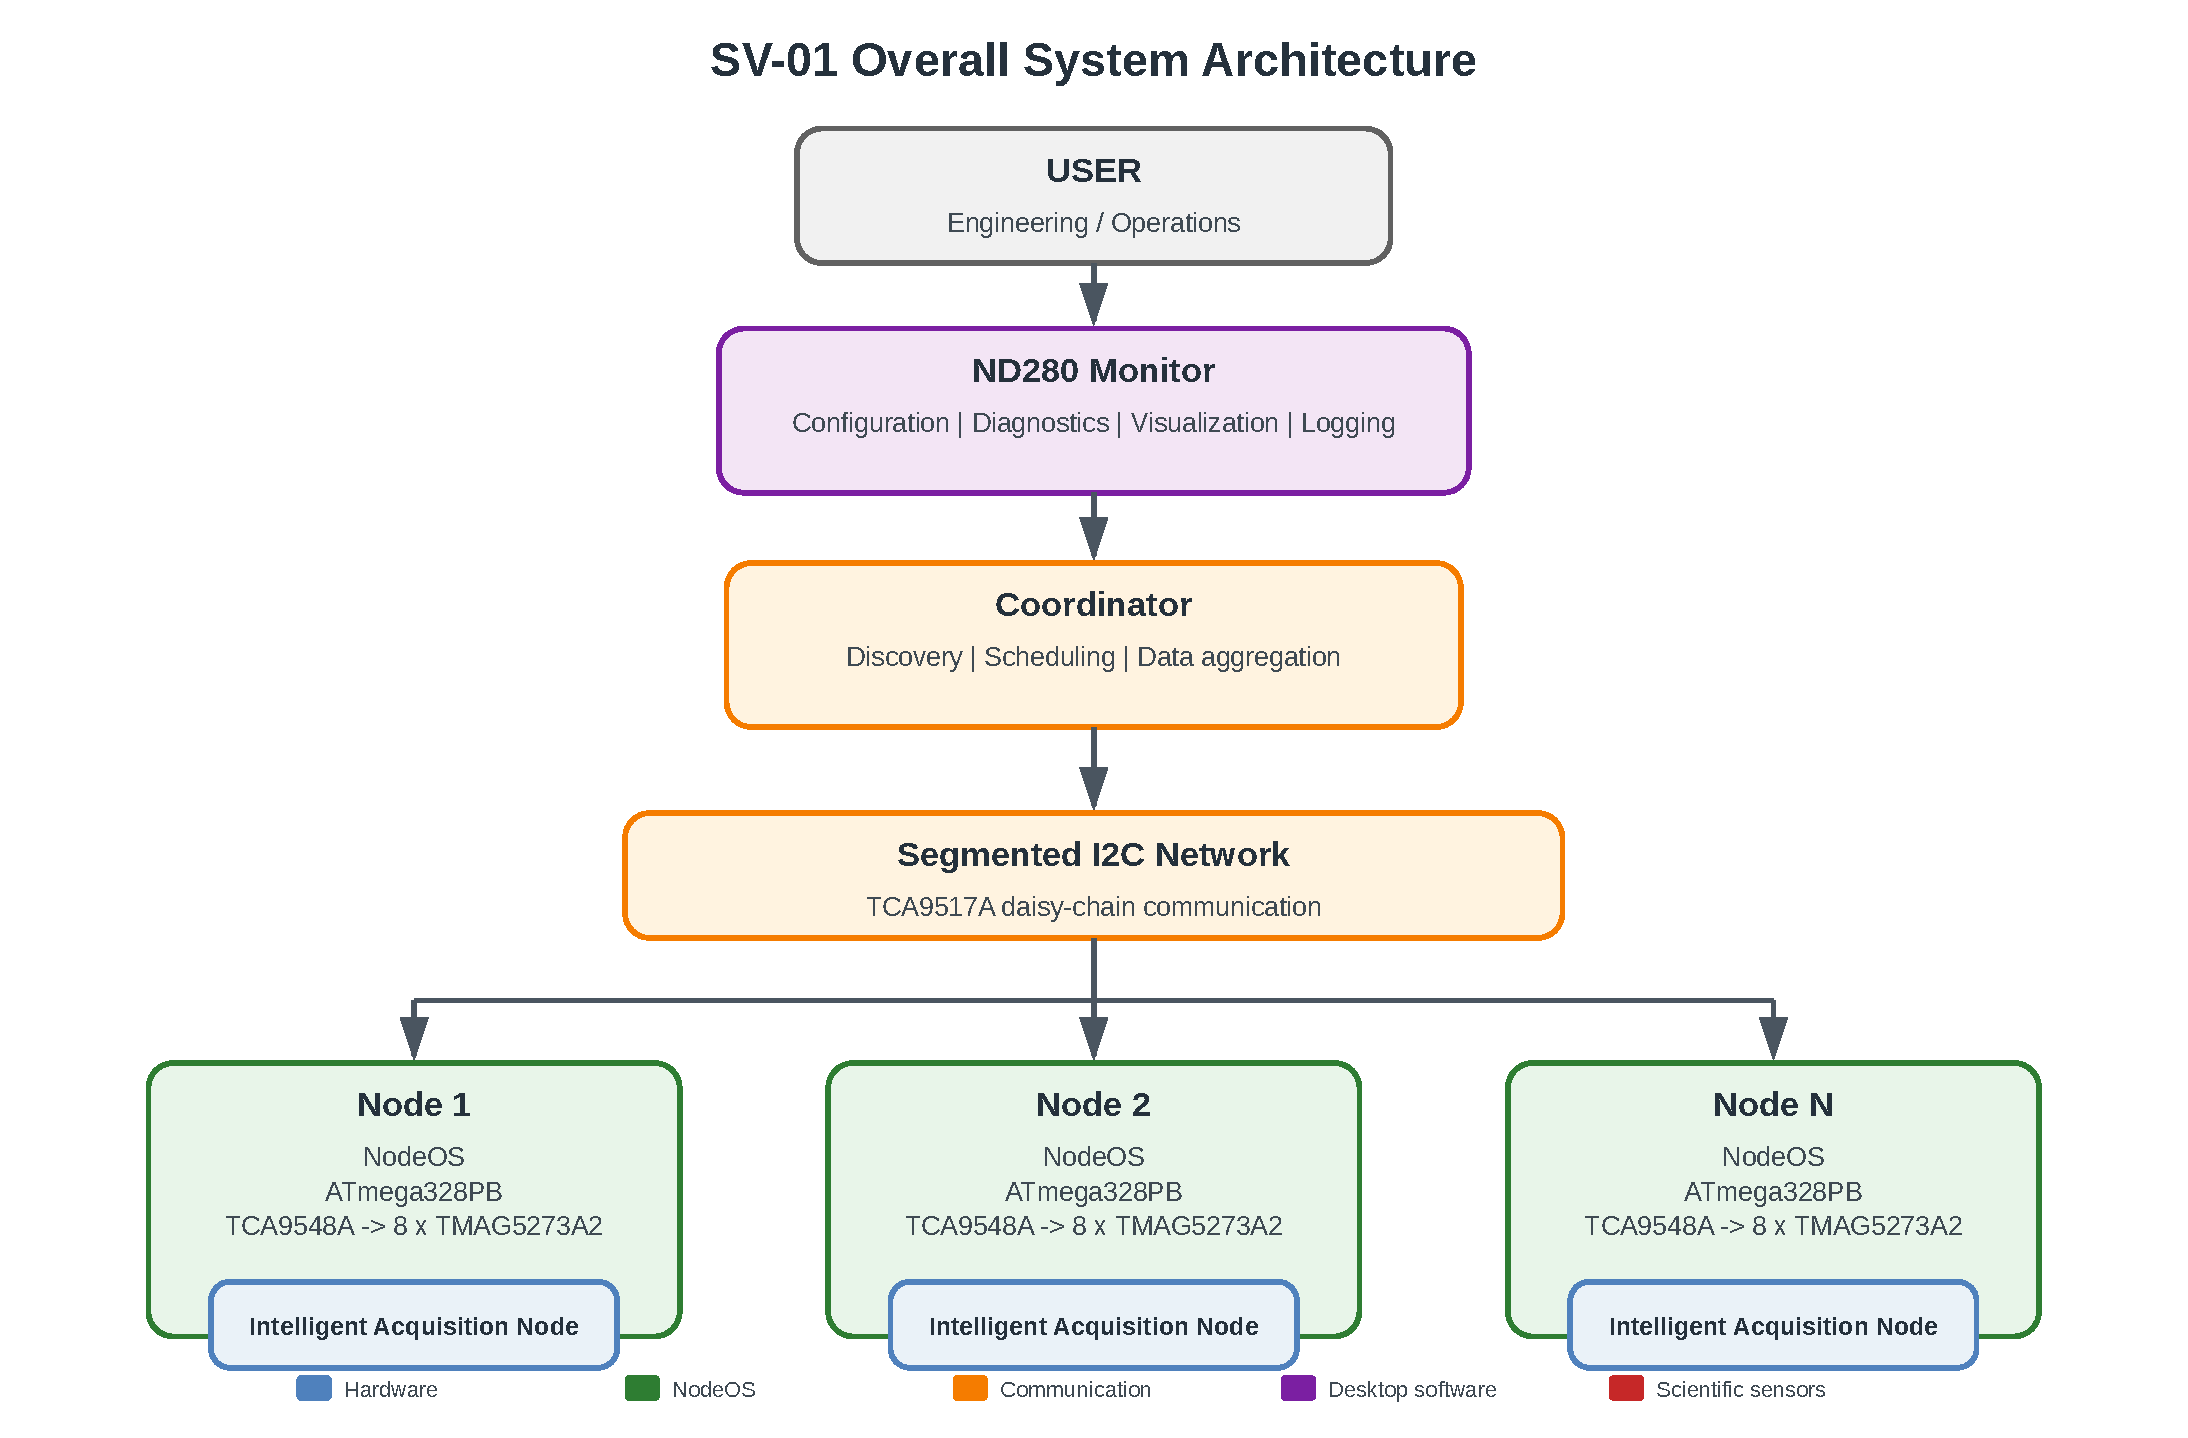
\includegraphics[width=0.98\textwidth]{SV01_Overall_System_Architecture.pdf}
  \caption{\textbf{SV-01 -- Overall System Architecture.} The monitoring system is composed of autonomous intelligent acquisition nodes connected through a segmented communication network. A Coordinator performs node discovery and data aggregation, while the ND280 Monitor provides the user-facing engineering interface.}
  \label{fig:sv01}
\end{figure}

The distributed architecture deliberately avoids direct sensor access from the PC. Each acquisition node is responsible for local sensor management, calibration and diagnostics. This limits the amount of information exchanged over the inter-board network and isolates sensor-specific implementation details from the higher-level system.

\section{Intelligent Acquisition Node}

The Intelligent Acquisition Node is the fundamental building block of the distributed architecture. It combines a local sensor-acquisition path with an independent inter-board communication path, both managed by the same microcontroller and NodeOS firmware.

\begin{figure}[htbp]
  \centering
  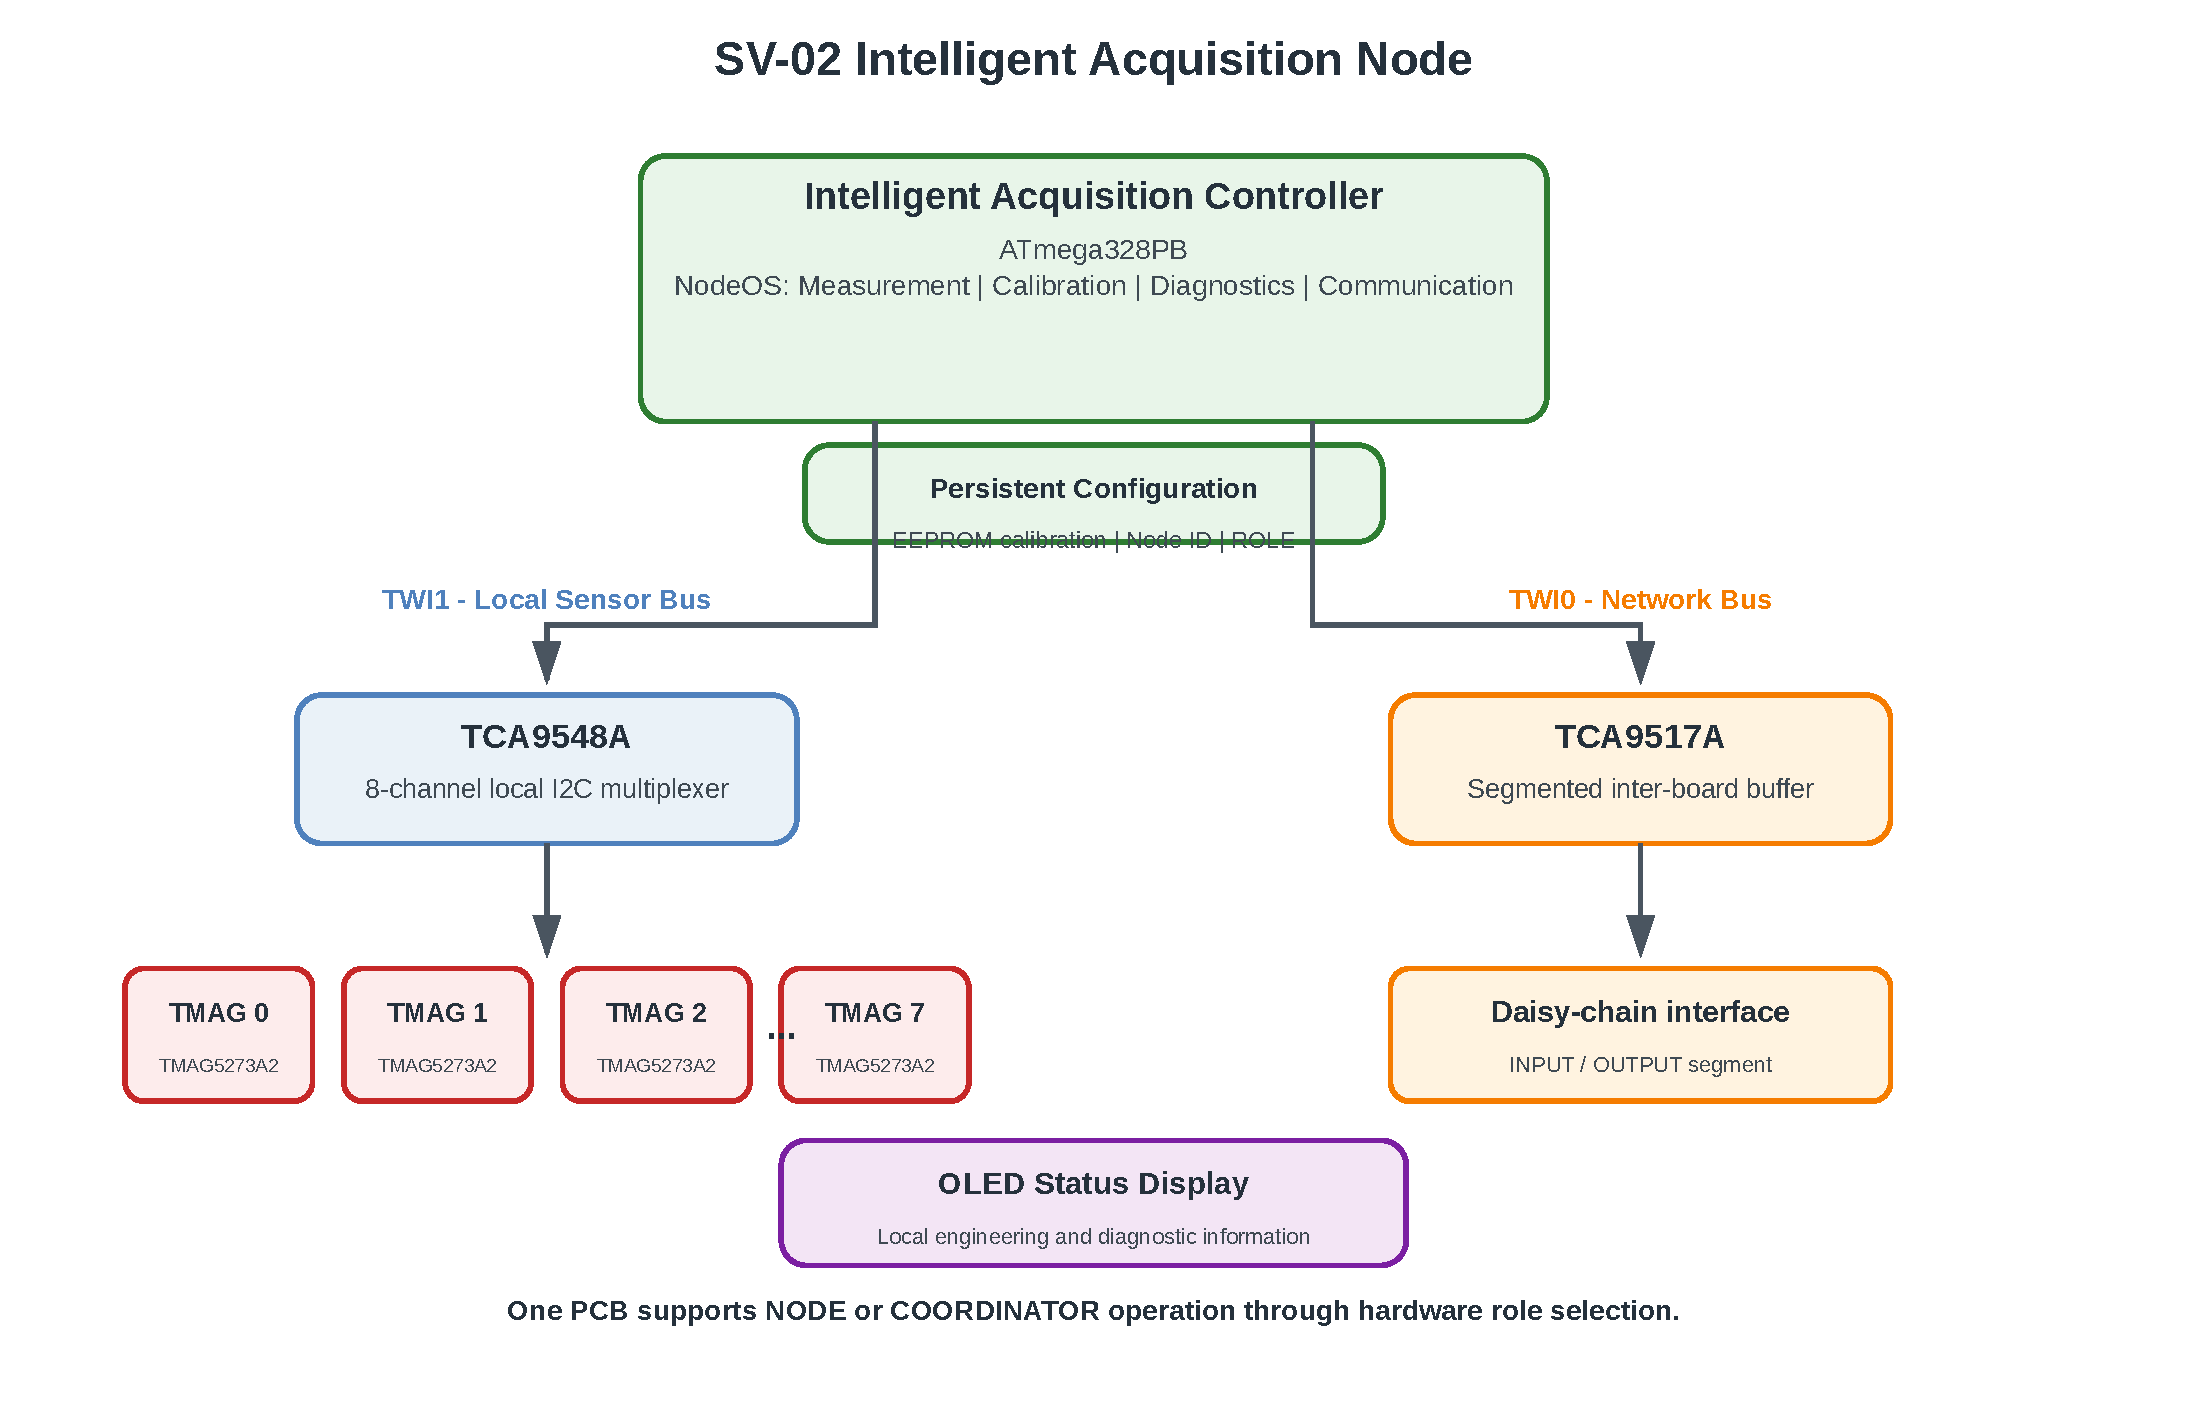
\includegraphics[width=0.96\textwidth]{SV02_Intelligent_Acquisition_Node.pdf}
  \caption{\textbf{SV-02 -- Intelligent Acquisition Node.} TWI1 is dedicated to the local magnetic-sensor subsystem through the TCA9548A multiplexer, while TWI0 is reserved for the segmented inter-board network through the TCA9517A. Hardware identity, operating role, OLED status and persistent calibration are local node resources.}
  \label{fig:sv02}
\end{figure}

The separation of TWI1 and TWI0 is a central architectural choice. Sensor acquisition remains independent of the communication topology, allowing the local measurement subsystem to evolve without redefining the external node interface. The same PCB can operate as a NODE or as a COORDINATOR, with the role selected by a dedicated hardware input.

\section{NodeOS Layered Architecture}

NodeOS provides the common embedded-software architecture used by the acquisition nodes. The application layer is intentionally isolated from microcontroller registers and device-specific peripheral details.

\begin{figure}[htbp]
  \centering
  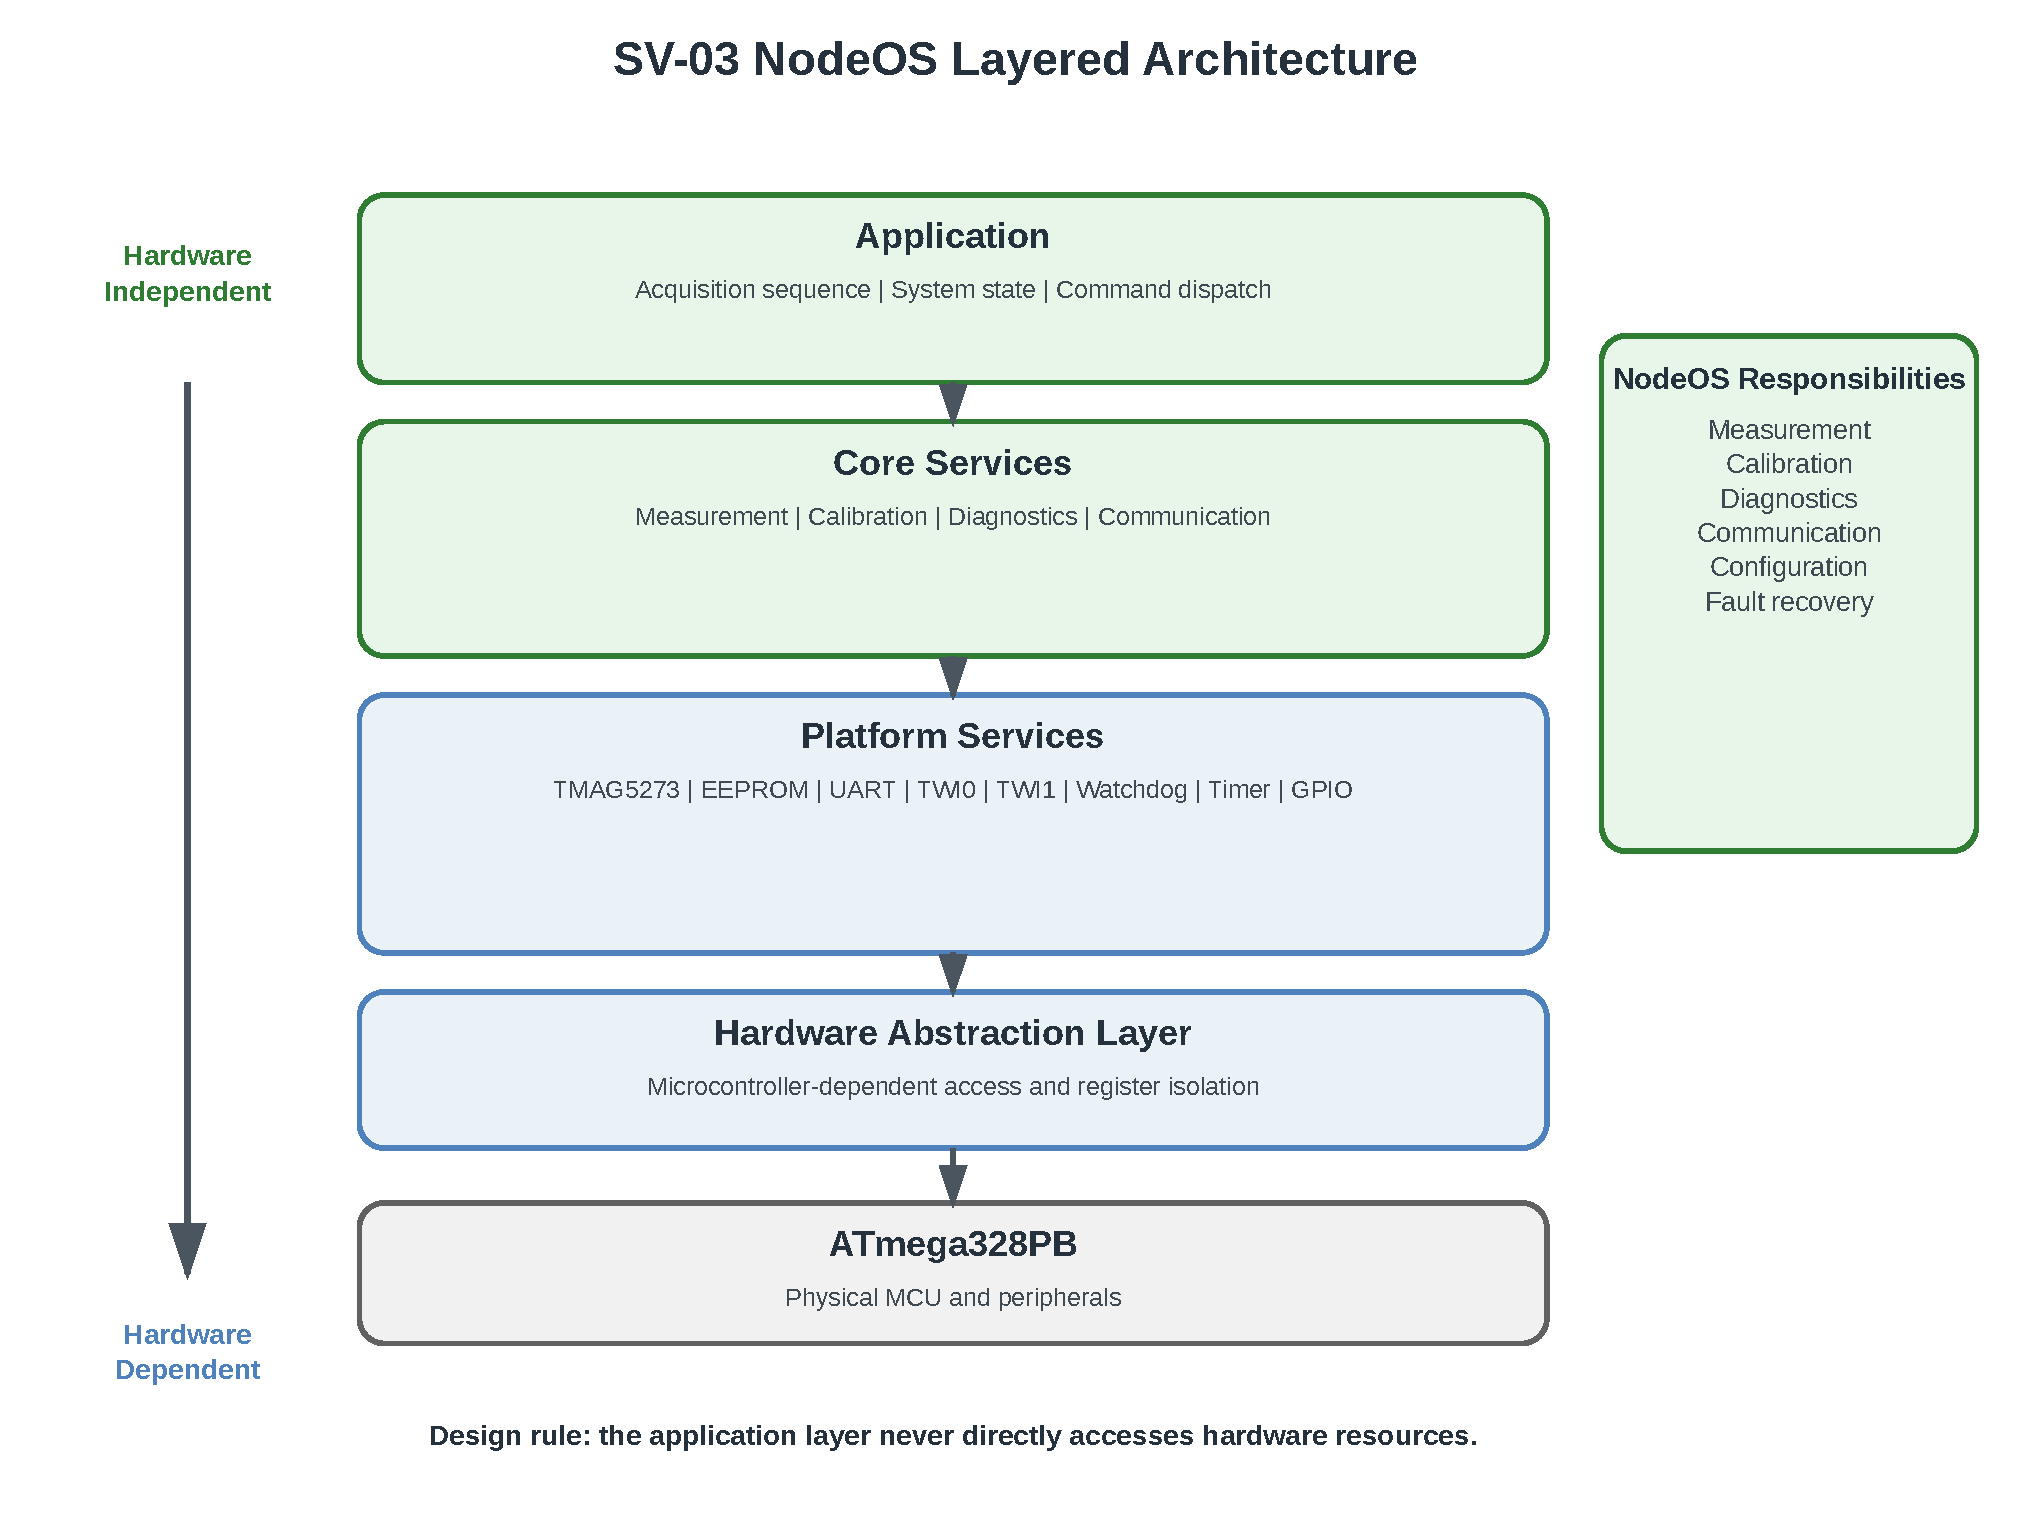
\includegraphics[width=0.92\textwidth]{SV03_NodeOS_Layered_Architecture.pdf}
  \caption{\textbf{SV-03 -- NodeOS Layered Architecture.} Hardware abstraction and platform services isolate the application and core services from the underlying microcontroller resources. This organization allows hardware evolution with limited impact on high-level acquisition logic.}
  \label{fig:sv03}
\end{figure}

At the highest level, the application controls the acquisition sequence and system state. Core services implement measurement, calibration, diagnostics and communication. Platform services provide access to persistent storage, watchdog supervision, transport and peripheral drivers. The hardware-abstraction layer contains the microcontroller-dependent interface.

This separation is a design constraint rather than only a coding convention: the application layer does not directly access hardware resources.

\section{Measurement Processing Workflow}

The system converts a physical magnetic-field quantity into validated and traceable scientific information through a deterministic sequence of processing steps.

\begin{figure}[htbp]
  \centering
  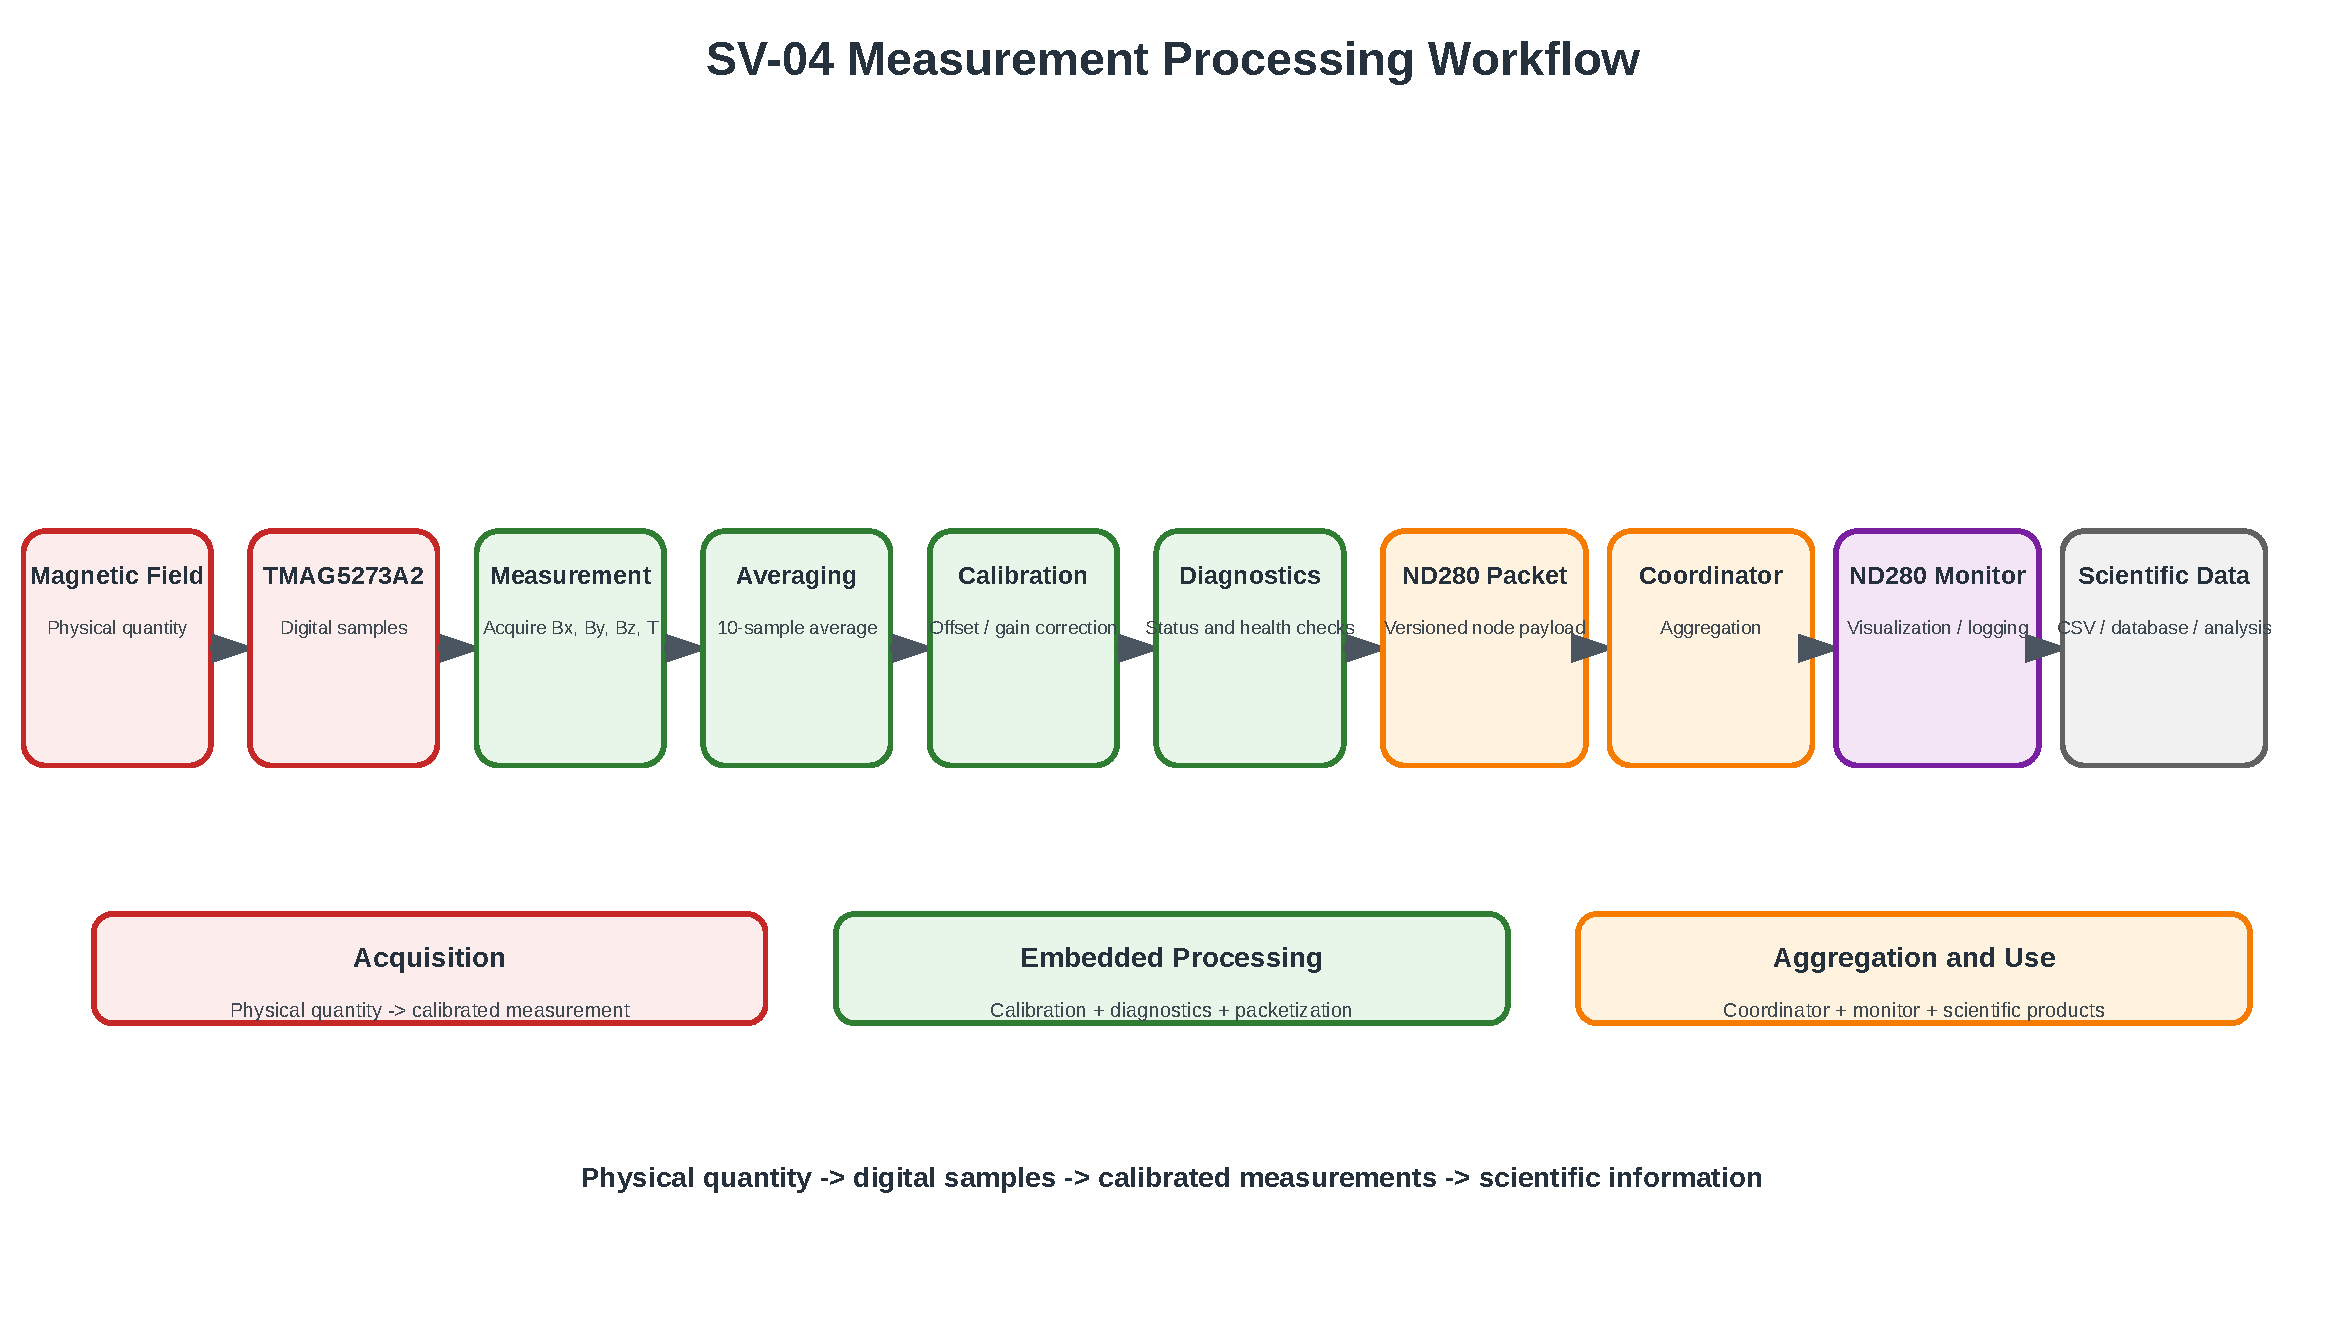
\includegraphics[width=0.98\textwidth]{SV04_Measurement_Processing_Workflow.pdf}
  \caption{\textbf{SV-04 -- Measurement Processing Workflow.} Transformation of the physical magnetic field into validated scientific information through acquisition, averaging, calibration, diagnostics, protocol framing, coordinator aggregation and desktop-level visualization or storage.}
  \label{fig:sv04}
\end{figure}

The TMAG5273A2 converts the local magnetic field and sensor temperature into digital samples. NodeOS performs acquisition, averaging and calibration, checks diagnostic status and constructs the measurement representation exposed to the communication layer. In the distributed system, the Coordinator aggregates measurements from multiple nodes before they are presented by the ND280 Monitor or stored as scientific data products.

This workflow preserves a clear distinction between raw sensor information, calibrated node-level measurements and higher-level aggregated data.

\section{Engineering Evolution}

The system has been developed incrementally. Each development stage was used to validate the assumptions required for the following stage rather than introducing all hardware and software complexity simultaneously.

\begin{figure}[p]
  \centering
  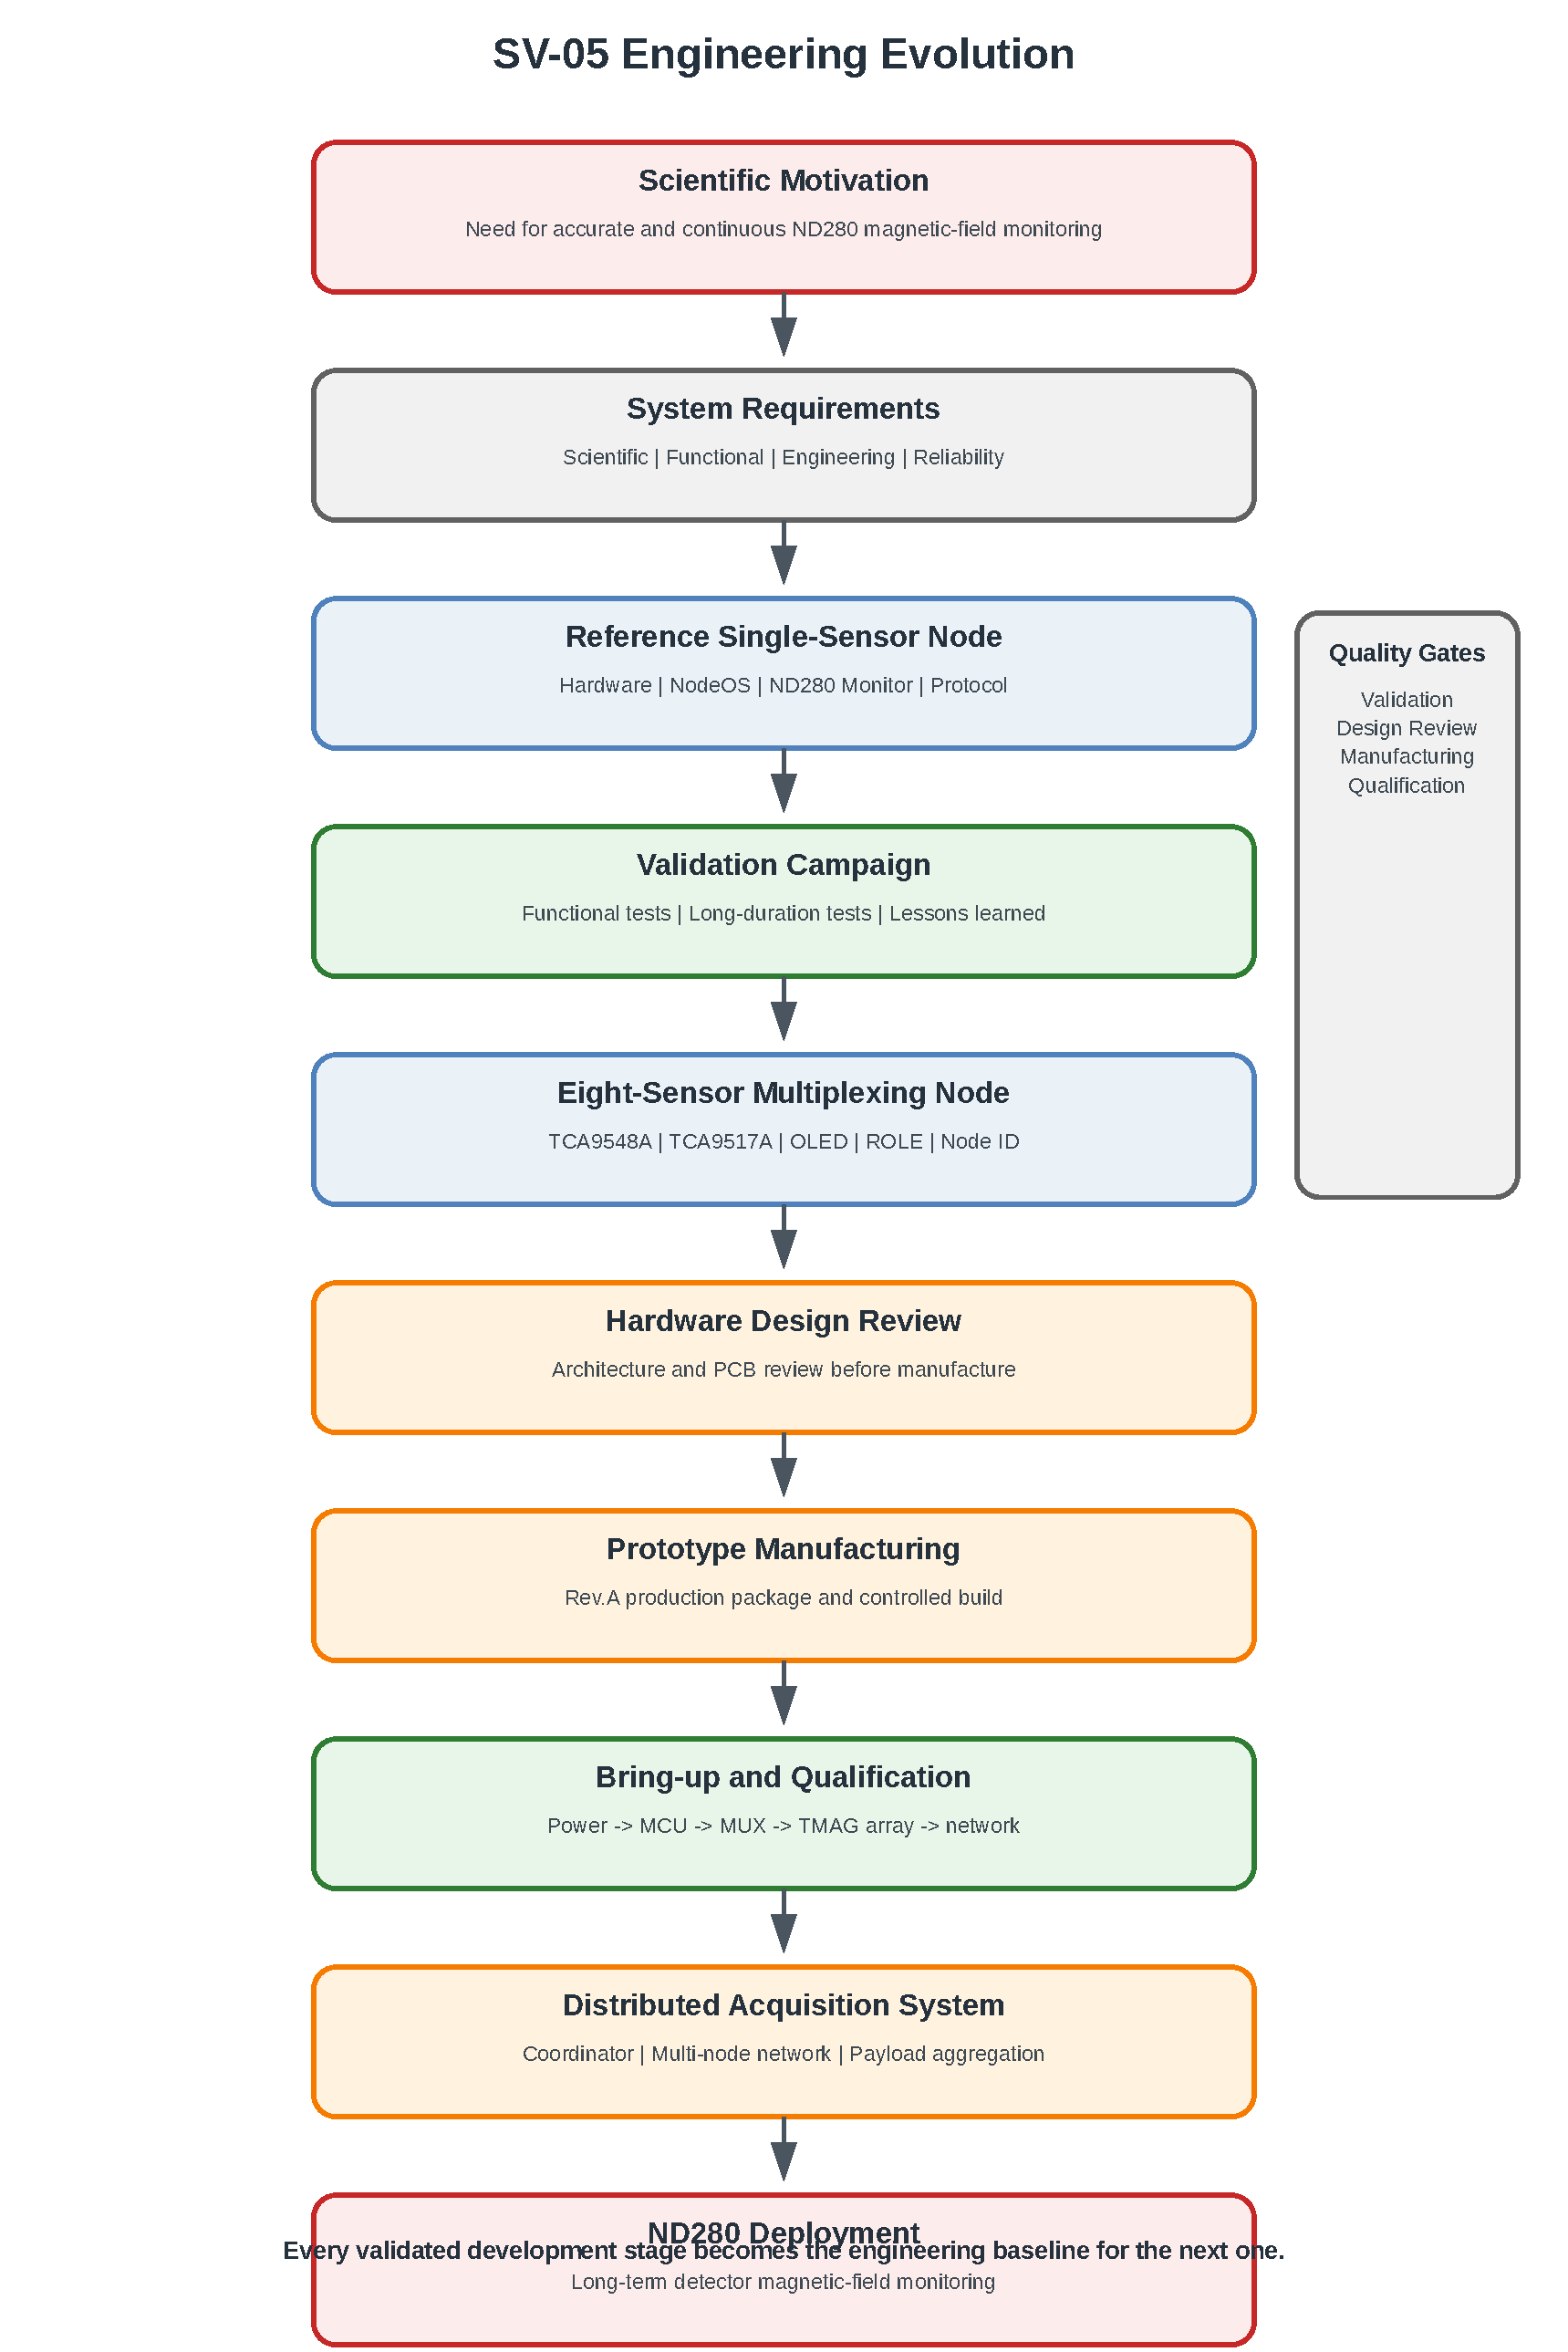
\includegraphics[height=0.80\textheight]{SV05_Engineering_Evolution.pdf}
  \caption{\textbf{SV-05 -- Engineering Evolution.} Each validated development stage generates engineering knowledge and deliverables that become the baseline for the following system revision. The approach couples incremental development with validation, design review and qualification.}
  \label{fig:sv05}
\end{figure}

The Reference Single-Sensor Node first validated the complete acquisition chain. The resulting hardware, NodeOS firmware, communication protocol and ND280 Monitor then formed the reference platform for the Eight-Sensor Multiplexing Node. The Rev.A design adds local multiplexing and segmented inter-board communication without abandoning the validated architectural principles.

The next stage is prototype manufacturing and bring-up of the Eight-Sensor Multiplexing Node, followed by multi-board validation and Coordinator development. This process can be summarized by the following engineering principle:

\begin{quote}
\emph{Every validated development stage generates engineering knowledge that becomes the foundation of the following system revision.}
\end{quote}

\section{Summary}

The System Views establish the common architectural vocabulary used throughout this report. The monitoring infrastructure is built from autonomous intelligent nodes; local sensor acquisition is separated from inter-board communication; NodeOS isolates high-level behaviour from hardware implementation; and measurement information is processed through a deterministic chain before aggregation and visualization.

The following chapter describes the Reference Single-Sensor Node, which was used to validate these principles before increasing hardware complexity.

\chapter{Reference Single-Sensor Node}
\label{chap:reference-node}

The Reference Single-Sensor Node represents the engineering baseline of the ND280 Magnetic Field Monitoring System. Its objective was not to implement the final detector hardware, but to validate the complete acquisition chain before introducing multiplexing and distributed communication.

The platform was used to validate hardware operation, magnetic-field acquisition, persistent calibration, NodeOS, the serial communication protocol, the ND280 Monitor, watchdog recovery and long-duration operational behaviour. Every subsequent hardware revision is derived from the architecture validated on this reference platform.

\section{Engineering Objectives}

The first development stage was intentionally limited to one magnetic sensor. This reduced hardware complexity while preserving all functions required to exercise the complete system from the physical measurement to the desktop application.

The Reference Platform was required to validate:
\begin{itemize}[leftmargin=*]
  \item acquisition of the three magnetic-field components and sensor temperature;
  \item operation of the TMAG5273A2 sensor and the ATmega328PB TWI interface;
  \item the NodeOS layered firmware architecture;
  \item hardware node identification;
  \item persistent calibration in EEPROM;
  \item watchdog supervision and reset-cause diagnostics;
  \item deterministic serial command handling;
  \item the ND280 communication packet format;
  \item the ND280 Monitor desktop application;
  \item long-duration acquisition and logging.
\end{itemize}

The goal was therefore to establish a stable engineering reference, not merely to demonstrate that a magnetic sensor could be read.

\section{Reference Platform Architecture}

\begin{figure}[htbp]
  \centering
  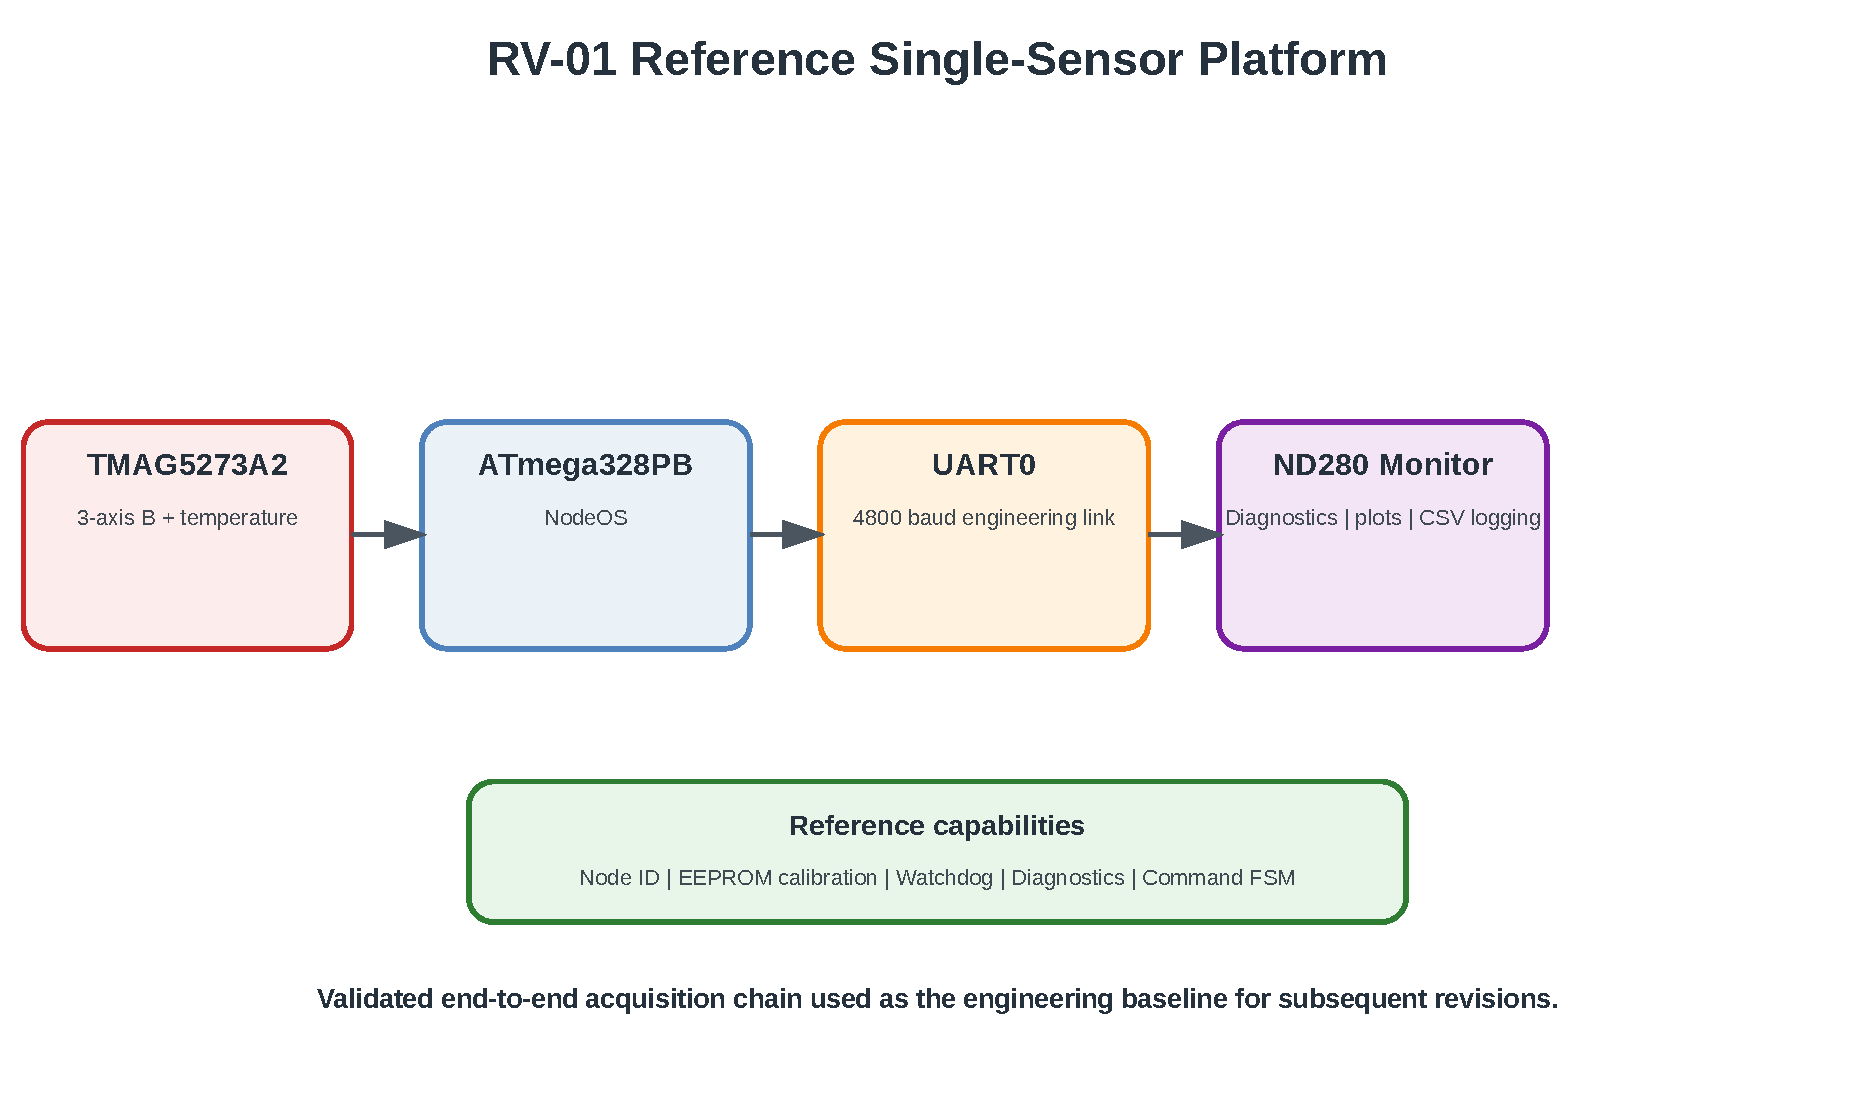
\includegraphics[width=0.88\textwidth]{RV01_Reference_Single_Sensor_Platform.pdf}
  \caption{\textbf{RV-01 -- Reference Single-Sensor Platform.} The reference acquisition chain couples one TMAG5273A2 sensor to the ATmega328PB running NodeOS and exposes the resulting measurements and diagnostics to the ND280 Monitor through UART.}
  \label{fig:rv01}
\end{figure}

The hardware architecture was kept deliberately simple. The ATmega328PB provides the embedded processing and peripheral interfaces, while the TMAG5273A2 provides three-axis magnetic-field and temperature measurements. The sensor is operated in the A2 range configuration used by the project, corresponding to a full-scale magnetic range of approximately \SI{266}{mT}.

The reference firmware configuration uses ten samples per reported measurement and a \SI{100}{ms} interval between samples. The measured values are averaged before calibration and packet generation. During the validation campaign the node communicated with the engineering PC interface through UART0 at 4800 baud.

The board includes hardware Node ID selection, non-volatile calibration storage and watchdog supervision. These functions were introduced at the reference stage because they were considered architectural requirements for the later distributed system rather than optional debugging features.

\section{NodeOS Integration}

The Reference Platform was the first complete hardware implementation of NodeOS. The firmware architecture separates application behaviour, reusable services, platform services and hardware-dependent access.

On the reference node, NodeOS provides:
\begin{itemize}[leftmargin=*]
  \item TMAG5273A2 initialization and measurement acquisition;
  \item sample averaging;
  \item calibration offset and gain application;
  \item EEPROM persistence and calibration-state reporting;
  \item hardware Node ID management;
  \item UART packet generation and command reception;
  \item diagnostics and internal counters;
  \item watchdog servicing and reset-cause reporting.
\end{itemize}

Developing and stabilizing these services before introducing the eight-channel multiplexer substantially reduced the risk of mixing firmware-architecture problems with new hardware-integration problems.

\section{Communication Architecture}

The reference node uses UART0 as its engineering communication interface. Measurement data are transmitted using the \texttt{\$ND280} packet family, while diagnostic and calibration information use dedicated response families such as \texttt{\$ND280DIAG}, \texttt{\$ND280CAL} and \texttt{\$ND280RSP}.

The command receiver evolved during validation. Early line-based parsing could interpret serial noise, echoes or unrelated traffic as commands. This behaviour was addressed by introducing a deterministic finite-state-machine parser in NodeOS v0.5.3-alpha1.

Commands are explicitly framed by the colon character. Examples include:
\begin{verbatim}
:HELP
:INFO
:DIAG
:CAL READ
:DIAG WDT TEST
\end{verbatim}

Input that does not belong to a valid command frame is ignored. The same rule is implemented by the ND280 Monitor transport layer, which adds the command prefix before transmission.

\section{Validation Campaign}

The Reference Platform was subjected to repeated functional tests and extended unattended acquisition runs. Validation covered the sensor interface, calibration persistence, watchdog recovery, serial communication, command parsing, diagnostics and desktop logging.

A representative long-duration run reached an uptime of 68,395 seconds (approximately 19 hours). At the end of the run the diagnostic counters reported 49,425 successful measurements, zero measurement failures, zero TWI errors and zero EEPROM errors.

\begin{table}[htbp]
\centering
\caption{Representative Reference Node long-duration validation results.}
\label{tab:reference-validation}
\begin{tabular}{lr}
\toprule
Parameter & Observed value \\
\midrule
Uptime & 68,395 s \\
Successful measurements & 49,425 \\
Measurement failures & 0 \\
TWI errors & 0 \\
EEPROM errors & 0 \\
\bottomrule
\end{tabular}
\end{table}

The run demonstrated stable sensor acquisition and persistence behaviour. UART receive robustness was treated as a separate engineering issue: receive-overflow and parser behaviour observed during earlier tests led to UART hardening and ultimately to the finite-state-machine command parser. The corrected firmware was subsequently exercised with diagnostic commands without disturbing normal measurement acquisition.

Watchdog functionality was also verified explicitly using the diagnostic watchdog test command. The firmware acknowledged the test, intentionally stopped servicing the watchdog and restarted with the reset cause correctly reported as \texttt{WATCHDOG}. This verified both the recovery mechanism and the associated diagnostics.

\section{Engineering Lessons Learned}

The Reference Platform produced several design decisions that directly influenced the later Eight-Sensor Multiplexing Node.

\subsection*{Validate the complete acquisition chain before increasing hardware complexity}
The single-sensor platform allowed sensor, firmware, protocol and desktop-software problems to be isolated and corrected without the additional variables introduced by multiplexing or multi-board networking.

\subsection*{Firmware architecture must precede hardware evolution}
NodeOS was stabilized before the eight-sensor hardware was introduced. The new board can therefore extend the measurement service instead of requiring a complete firmware redesign.

\subsection*{Diagnostics are part of the system architecture}
Watchdog counters, reset flags, TWI statistics, measurement counters and EEPROM status proved essential during long-duration testing. They are retained as permanent services rather than temporary debug instrumentation.

\subsection*{Command processing must be deterministic}
Serial command reception must be explicitly framed and independent of arbitrary serial traffic. The finite-state-machine parser and mandatory colon prefix were introduced as a direct consequence of validation observations.

\subsection*{Calibration and identity must survive operational cycles}
Persistent EEPROM calibration and hardware-defined Node ID prevent configuration ambiguity after power cycling and simplify replacement or reinstallation of a node.

\subsection*{Long-duration tests are required before freezing the next hardware stage}
Short functional tests demonstrated correctness, but unattended operation exposed communication and recovery behaviours that were not visible during bring-up. Long-duration validation therefore became a required gate before subsequent hardware evolution.

\section{Summary}

The Reference Single-Sensor Node established the validated baseline of the ND280 Magnetic Field Monitoring System. It demonstrated that the sensor, NodeOS firmware, communication protocol, calibration storage, watchdog diagnostics and ND280 Monitor could operate as one coherent acquisition chain over extended periods.

The resulting engineering knowledge and validated software architecture formed the basis of the Eight-Sensor Multiplexing Node described later in this report.

\chapter{NodeOS Firmware}

NodeOS is the embedded firmware architecture developed for the acquisition nodes. It separates hardware abstraction, device drivers, services and application logic.

The current validated baseline includes magnetic-field and temperature acquisition, averaging, EEPROM calibration storage, diagnostics, watchdog recovery, reset-cause reporting and a deterministic finite-state-machine command parser.

\chapter{ND280 Monitor}

The ND280 Monitor is the Python desktop application used for commissioning, diagnostics, calibration, real-time visualization and CSV logging.

The monitor implements the command transport required by the NodeOS finite-state-machine parser and provides engineering access to node identity, diagnostics and calibration information.

\section{Operational View}

The application provides a unified view of the selected node, the magnetic-field and temperature trends, the NodeOS control panel, diagnostic responses and the raw serial stream. This makes it possible to correlate high-level monitoring information with the exact protocol traffic produced by the embedded node.

Figure~\ref{fig:monitor_long_run} shows the ND280 Monitor during an extended acquisition run of the Reference Single-Sensor Node. The screenshot documents simultaneous visualization of the three magnetic-field components, sensor temperature, node identity, packet continuity and the NodeOS diagnostic response.

\begin{figure}[p]
    \centering
    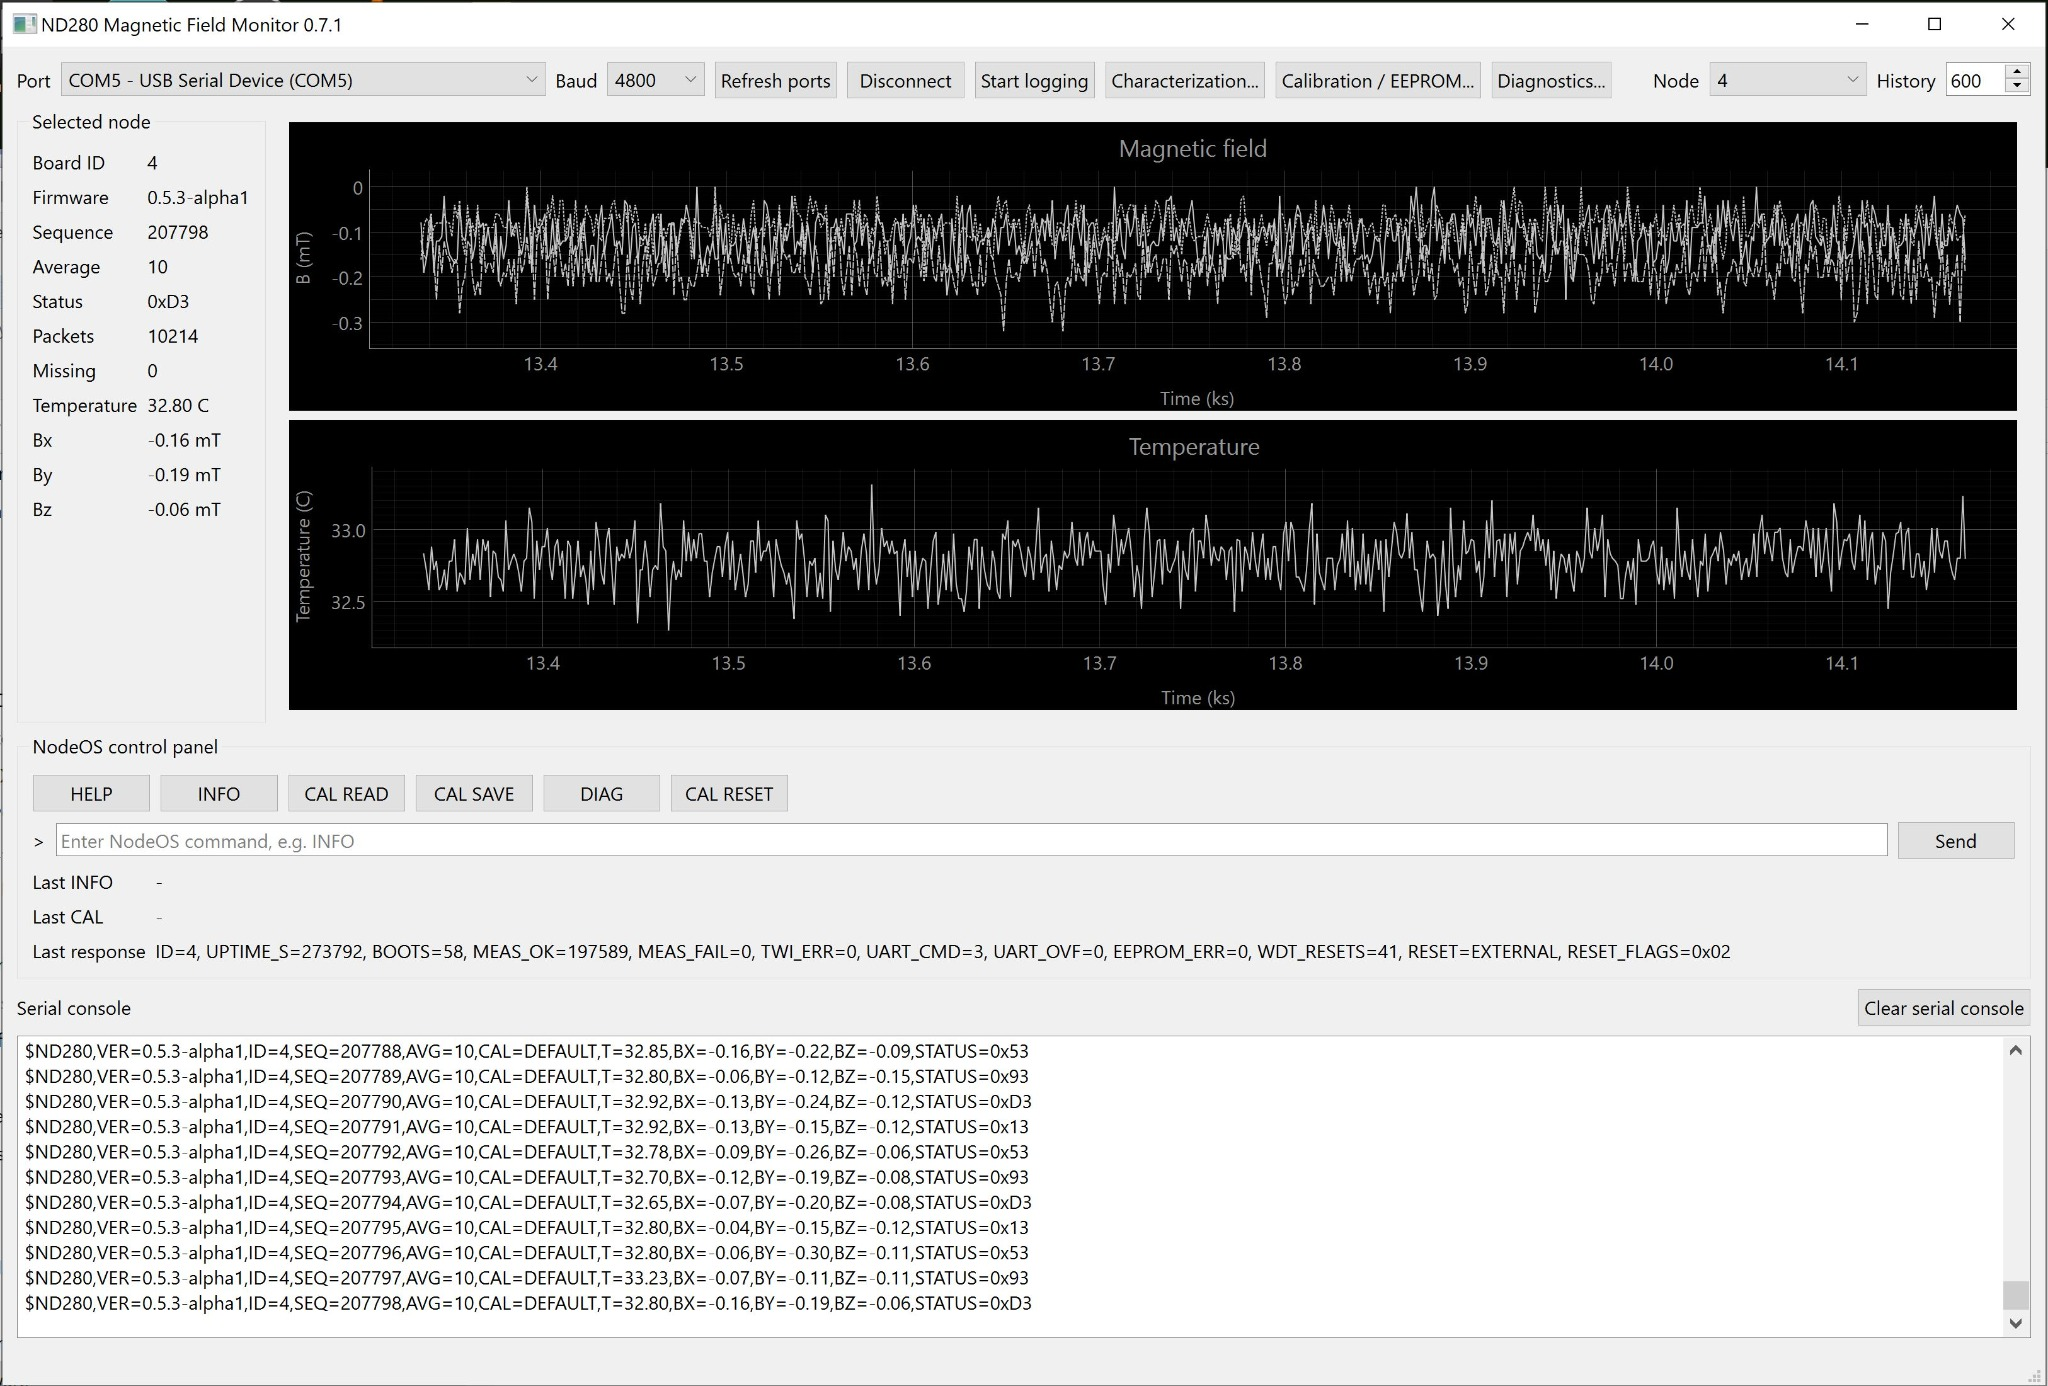
\includegraphics[width=\textwidth]{SW01_ND280_Monitor_Long_Duration_Run.jpg}
    \caption{ND280 Monitor during an extended long-duration acquisition test of the Reference Single-Sensor Node. At the time of the screenshot, Node~4 running NodeOS v0.5.3-alpha1 reported an uptime of 273792~s, 197589 successful measurements, no measurement failures, no TWI errors, no UART receive overflow and no EEPROM errors. The monitor simultaneously displays magnetic-field and temperature trends, node status, the diagnostic response and the raw NodeOS serial stream.}
    \label{fig:monitor_long_run}
\end{figure}

\section{Engineering Role}

The ND280 Monitor is not only a visualization tool. During development it has been used as the primary engineering interface for firmware bring-up, command testing, EEPROM and calibration operations, long-duration logging and diagnostic inspection. Its behaviour therefore forms part of the validated end-to-end acquisition chain described in this report.

\chapter{Eight-Sensor Multiplexing Node}

The Eight-Sensor Multiplexing Node extends the Reference Node by adding a TCA9548A local I\textsuperscript{2}C multiplexer and up to eight TMAG5273A2 sensors.

The Rev.A hardware also includes a TCA9517A for segmented inter-board communication, an OLED display, a hardware NODE/COORDINATOR role selector, hardware node identification and dedicated reset/enable control signals.

\section{Rev.A Hardware Realization}

Figure~\ref{fig:revA_render} shows the current three-dimensional rendering of the Eight-Sensor Multiplexing Node Rev.A. The rendering is included to connect the functional architecture introduced in Chapter~4 with the physical hardware implementation. The eight TMAG sensor positions are distributed along the lower edge of the board, while the controller, local multiplexer, OLED display, configuration elements and inter-board connectors are integrated on the same PCB.

\begin{figure}[p]
    \centering
    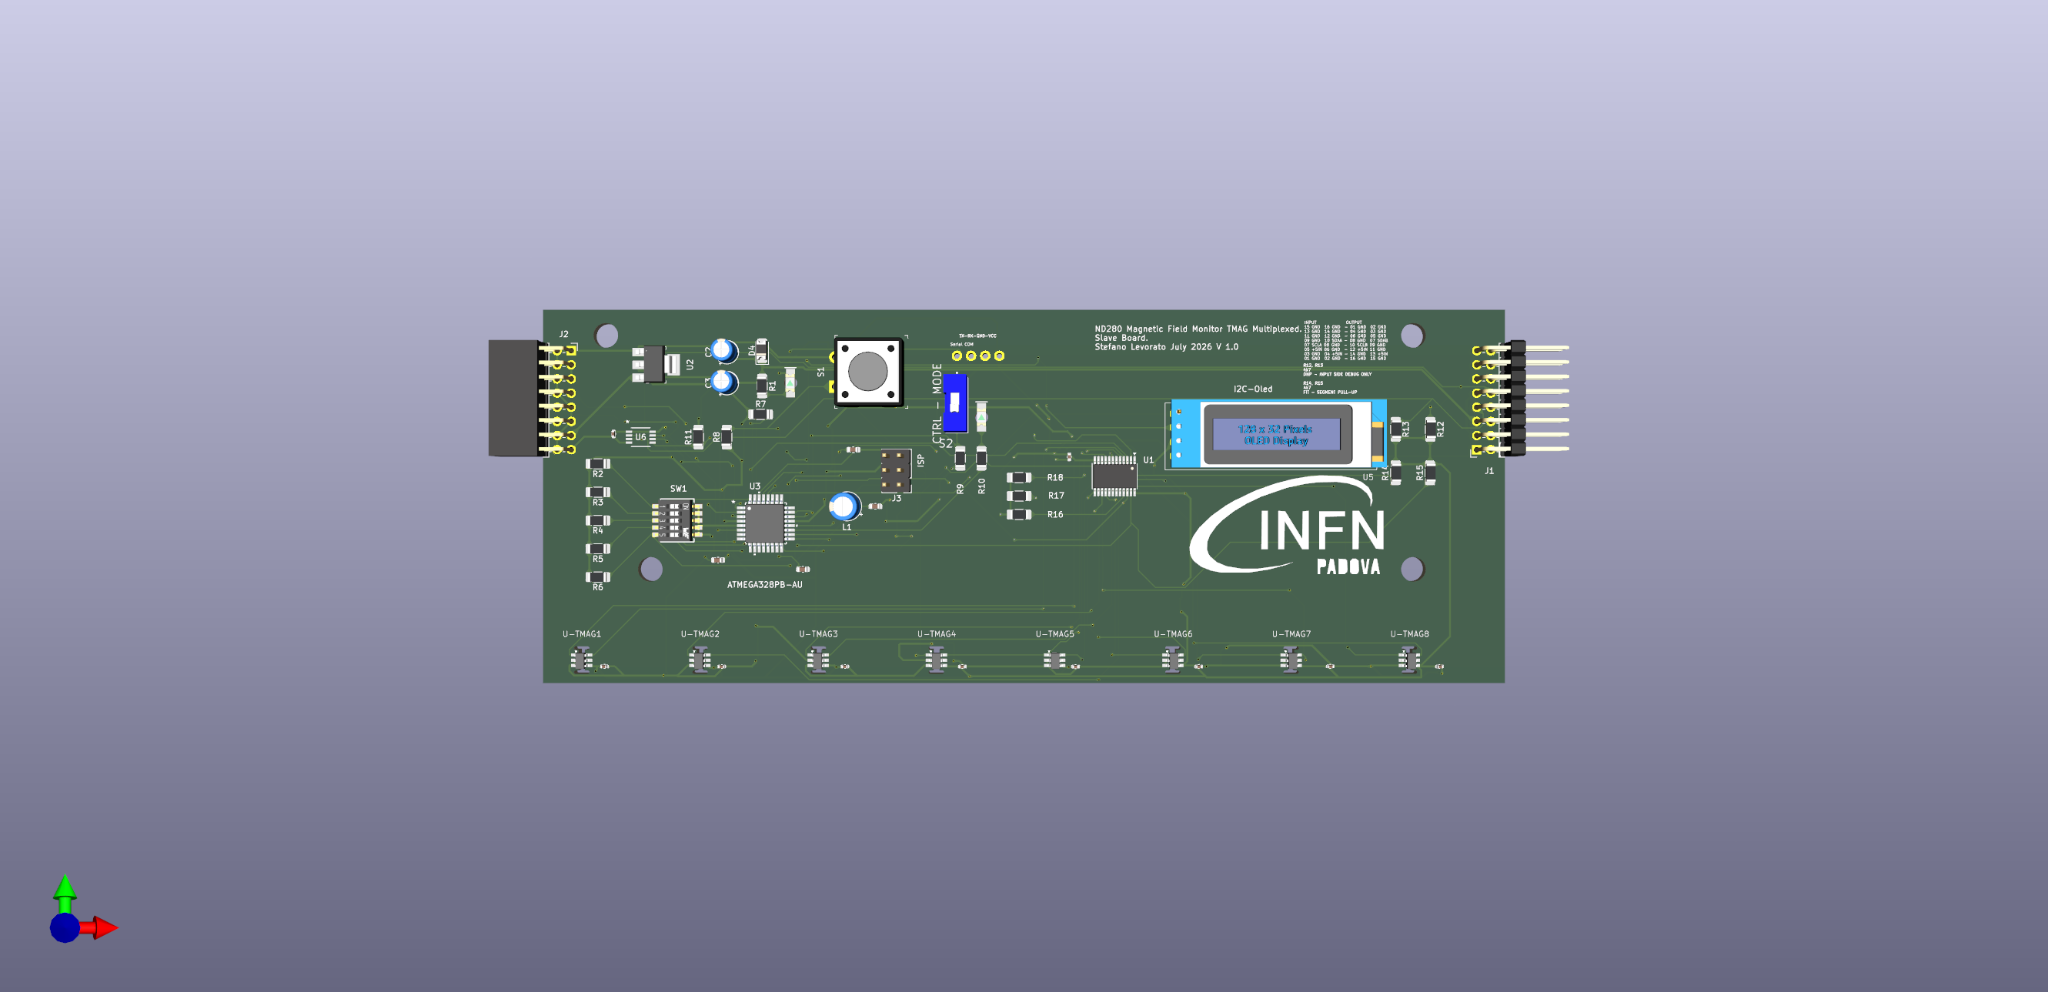
\includegraphics[width=\textwidth]{HV01_Eight_Sensor_Multiplexing_Node_Render.png}
    \caption{Three-dimensional rendering of the Eight-Sensor Multiplexing Node Rev.A. The board integrates the ATmega328PB controller, TCA9548A local sensor multiplexer, TCA9517A segmented inter-board interface, OLED display, hardware configuration elements and eight TMAG5273A2 sensor positions on a single PCB.}
    \label{fig:revA_render}
\end{figure}

\section{Architectural Continuity}

The Rev.A board preserves the architectural principles validated on the Reference Single-Sensor Node. Local acquisition remains under NodeOS control, while the additional hardware extends the number of sensors and introduces the physical infrastructure required for distributed operation. This allows the new board to be treated as an evolution of the validated reference platform rather than as an independent redesign.

\chapter{Distributed Acquisition System}

The distributed architecture is intended to support multiple acquisition boards connected in a segmented daisy chain.

Each NODE performs local acquisition and exposes processed measurements to the upstream COORDINATOR. The COORDINATOR scans the configured node-address range, maintains a node table and aggregates measurements into a coherent higher-level payload.

The long-term target is a system of up to 32 acquisition boards, corresponding to a maximum of 256 magnetic sensors.

\chapter{Communication Protocol}

The current NodeOS command protocol uses a mandatory colon prefix. Measurement and diagnostic responses use the \texttt{\$ND280} packet family.

Examples include:
\begin{verbatim}
:HELP
:INFO
:DIAG
:CAL READ
\end{verbatim}

The protocol will be extended for multi-sensor and multi-board operation while preserving explicit versioning.

\chapter{Validation Campaign}

The Reference Node has been exercised through functional tests and long-duration acquisition runs.

\section{Initial Long-Duration Test}

A representative long-duration test reached an uptime of 68,395 seconds, with 49,425 successful measurements, zero measurement failures, zero TWI errors and zero EEPROM errors.

UART receive robustness was subsequently improved through the finite-state-machine command parser used in NodeOS v0.5.3-alpha1.

\section{Extended Long-Duration Test}

A later extended acquisition run provided a substantially longer operational sample. As documented in Figure~\ref{fig:monitor_long_run}, the Reference Single-Sensor Node reached an uptime of 273792 seconds (approximately 76 hours). At the captured point the diagnostic counters reported 197589 successful measurements, zero measurement failures, zero TWI errors, zero UART receive overflows and zero EEPROM errors.

The ND280 Monitor simultaneously reported zero missing packets for the displayed acquisition sequence. This extended run provides additional evidence that the acquisition, TWI communication, EEPROM handling, command transport and monitoring chain can operate continuously over multi-day periods without the error modes observed during the earlier UART parser development phase.

These results validate the Reference Node as an engineering baseline. Final noise, offset, thermal behaviour, absolute calibration and distributed-bus performance remain to be qualified on the Eight-Sensor Multiplexing Node and on the final detector hardware.

\chapter{Conclusions and Future Developments}

The Reference Single-Sensor Node has validated the core hardware, firmware and software architecture.

The next project phase is the prototype manufacture and staged bring-up of the Eight-Sensor Multiplexing Node Rev.A, followed by progressive validation of the inter-board communication architecture and the coordinator functionality.


\appendix
\chapter{Hardware Revision History}

\begin{tabular}{llll}
\toprule
Revision & Date & Status & Description \\
\midrule
Reference Node & 2026 & Validated & Single-sensor reference platform \\
Rev.A & 2026 & Prototype design & Eight-sensor multiplexing board \\
\bottomrule
\end{tabular}

\chapter{Firmware Revision History}

\begin{tabular}{lll}
\toprule
Version & Status & Main content \\
\midrule
0.5.2-alpha1a & Stable baseline & Watchdog and UART RX hardening \\
0.5.3-alpha1 & Stable baseline & Finite-state-machine command parser \\
\bottomrule
\end{tabular}

\chapter{Protocol Reference}

\section{Command Prefix}
All NodeOS commands shall begin with the ASCII character `:'.

\section{Current Commands}
\begin{verbatim}
:HELP
:INFO
:DIAG
:DIAG WDT TEST
:CAL READ
:CAL OFFSET x y z
:CAL GAIN x y z
:CAL NOISE x y z
:CAL TEMP t
:CAL SAVE
:CAL RESET
\end{verbatim}

\chapter{Architecture Decision Record Index}

The Architecture Decision Records are maintained separately in the project repository. The TDR references the accepted decisions relevant to each subsystem.


\bibliographystyle{unsrt}
\bibliography{bibliography/references}
\end{document}
